\documentclass[12pt]{book}
\usepackage{fullpage,setspace}

\usepackage{tocbibind}

% Change ToC title
\renewcommand\contentsname{Table of Contents}

% Section numbering only of main sections
\setcounter{secnumdepth}{1}

% Put an index into this manual
\usepackage{makeidx}
\makeindex


\usepackage{sidecap}
\usepackage{subfig}
\usepackage{graphicx,amsmath,amssymb}
\usepackage{pstricks}
\usepackage{epic,eepic}
\usepackage{url}
\usepackage{listings}
\usepackage{longtable}
\usepackage{units}

% make sure to put this last!!
\usepackage[colorlinks]{hyperref}
\usepackage{breakurl}

\newcommand{\gui}[1]{``{\ttfamily #1}''}
\newcommand{\code}[1]{``{\ttfamily #1}''}
\newcommand{\macroline}[1]{``{\ttfamily #1}''}
\newcommand{\macrolinenoquotes}[1]{{\ttfamily #1}}
\newcommand{\selectordeselect}[0]{\macrolinenoquotes{Select} or \macrolinenoquotes{Deselect} }


% This is formatting for the source code and 
% other files in my paper
\lstset{numbers=left,columns=fixed}
\lstset{basicstyle=\ttfamily}
%\lstset{basicstyle=\ttfamily\small}
\lstset{language=csh}
\lstset{xleftmargin=3em,xrightmargin=3em}
\lstset{frame=tb}
%\lstset{commentstyle=\bfseries\color{black}\underbar}


\begin{document}

\title{X-ray Diffraction GUI Manual\footnote{The red text in this paper are links to other parts of the document or other webpages.}}
\date{\today}
\author{Joshua~Lande (\href{mailto:joshualande@gmail.com}{joshualande@gmail.com})}
\maketitle

\tableofcontents

\chapter{Tips and Tricks}
\index{Tips and Tricks}
\chapter{Tips and Tricks}

\section{Calibration}

The \gui{Calibration} tab can also be used to load
diffraction data into the program. The tab can
be used to calibrate diffraction data to determine the 
parameters that characterize the experiment. 
Diffraction data can be loaded using the \gui{Data File:} input. 
The program recognizes \macroline{mar2300}, \macroline{mar3450}, 
\index{Mar2300}\index{Mar3450}\index{MarCCD}\index{Tiff}
\macroline{mccd}, \macroline{tiff}, and \macroline{edf} data. 
Multiple files can be loaded into the program at the same
time using the file selector and the sum image is loaded.

This program characterizes a diffraction experiment 
according to the parameters:
\index{Calibration Parameters}
\index{X Center}\index{Y Center}
\index{Detector Distance}\index{$\alpha$}
\index{$\beta$}\index{Rotation}\index{Pixel Scale}
\begin{itemize}
    \item \gui{xc:}, \gui{yc:} - the $(x,y)$ pixel coordinate 
    on the detector where the incoming 
    x-ray beam would have hit the detector were there 
    no sample in the way (in pixels).
    \item \gui{d:} -- the distance from the sample to 
    the detector (in mm).
    \item \gui{E:} -- the energy of the incoming beam (in eV).
    \item \gui{alpha:}, \gui{beta:} \gui{R} -- 3 rotations of 
    the detector (in degrees).
    \item \gui{pl:} -- the pixel length of the detector - 
    the width of one pixel (in microns).
    \item \gui{ph:} -- The pixel height of the detector -
    the height of one pixel (in microns).
\end{itemize}
Before calibrating an image, three things must be done. 
First, the diffraction data must be loaded.
Second, a $Q$ data file with standard $Q$ values for the
sample must be loaded.
Third, an initial guess of the calibration parameters must be
loaded. A guess at the calibration parameters can sometimes
be found in the header of the diffraction file. These values
can be loaded into the program using the \gui{Get From Header} 
button.  The \gui{Do Fit} button will perform the calibration 
and find a best guess at the real experimental parameters.

The \gui{Work in Lambda} option in the \gui{Calibration} menu can
be used to make the program work with the x-ray's
wavelength instead of its energy. The calibration parameter 
\gui{$\lambda$:} will be used instead of \gui{E:}.

The \gui{Q Data:} input will load into the program standard $Q$ data files. 
This program stores several standard $Q$ files that can be selected
through the \gui{Standard Q} option of the \gui{Calibration} menu.

The calibration algorithm can be modified in a couple of ways.
The program finds peaks in the diffraction data by 
running from the center of the image out. 
The number of radial slices that the program uses
can be set with the \gui{Number of Chi?} input.
The \gui{Stddev?} input 
tells the program what ratio higher a peak must be than the 
standard deviation of the background near it for the
peak to be considered real. The higher the value, the more
picky the program is about finding legitimate peaks.

If some of the experimental parameters are known exactly, 
the \gui{Fixed?} check box associated with that variable 
will stop it from being refined when fitting. The pixel 
length and pixel height are never refined. 

To see how good the current calibration parameters are, 
the \gui{Draw Q Lines?} 
check box will make the program draw 
on the diffraction image lines of constant $Q$ specified
by the $Q$ data file. The $\Delta Q$ ranges specified in 
the $Q$ data file can be drawn using the \gui{Draw dQ Lines?} 
check box. The diffraction peaks that were found while
calibrating can be displayed using the \gui{Draw Peaks?} check box. 

The diffraction image can be zoomed into by left clicking
on the image, dragging the mouse, and then releasing.
The image can be unzoomed by right clicking on the image. 
The image can be panned across by shift clicking on the image 
and dragging. The image can be made bigger or smaller by 
resizing the window.

In the \gui{File} menu, the \gui{Save Image} option can be used 
to save the current diffraction file in several popular
image formats. The image will be saved with the current
zoom level and any $Q$ lines, $\Delta Q$ lines, peaks, or
masks drawn on it.

\section{Masking}
\index{Pixel Masking}

The program can ignore certain pixels in an image
when performing diffraction analysis. This can be done
using the \gui{Masking} tab.  Threshold masking can be 
used to ignore pixels above or below a certain value.
All pixels larger than a certain value can be masked 
using the \gui{Do Greater Than Mask?} check box
and specifying the value in the 
\gui{(Pixels Can't Be) Greater Than Mask:} input.
All pixels less than a certain value can be ignored 
using the \gui{Do Less Than Mask?} check box 
and specifying the value in the 
\gui{(Pixels Can't Be) Less Than Mask:} input.
The overloaded or underloaded pixels will show up
as a different color on the diffraction and cake images.
This color can be changed using the \gui{Color} buttons
near the other inputs.
When a threshold mask is applied, masked pixels
will not be used during an intensity integration.

The program can mask areas of the diffraction image
using polygon masks. The \gui{Do Polygon Mask?} check box 
will enable this. Any masks in the program
will be displayed over the diffraction data and cake images.
Any masked pixels will not be used during an intensity
integration. The \gui{Add Polygon} button can be used to 
draw new polygon masks. To draw a mask, simply push
the button, left click all the
nodes on the diffraction image except the last one, and
then right click the final node. 
The \gui{Remove Polygon} button can be used to 
remove polygons from the diffraction image. Simply push
the button and then click on the polygon that should be
removed. The \gui{Clear Mask} button will remove all
the polygons from the program. The \gui{Save Mask} button
and the \gui{Load Mask} button will save and load
polygons to and from a file.

\section{Caking}
\index{$\chi$}\index{$Q$}\index{Caking}

A cake is a plot of diffraction data in $Q$ vs.
$\chi$ space. $\chi$ is a measure of the angle around 
the incoming x-ray beam. By convention, $\chi$ is equal to 
$0\degrees$ to the right of the center of the image and
increases in a counterclockwise direction. 
The program needs to know a range and bin size in $Q$ and
$\chi$ in order to make a caked plot. The \gui{Do Cake} button
will create a cake and open a new window with the caked data in
it. The caked window can be interacted with just like
the diffraction window. There is a button called \gui{AutoCake} that 
picks a cake range with the whole diffraction image in it 
and then cakes the data. Any $Q$ lines, $\Delta Q$ lines,
and peaks that are drawn on the diffraction image
will also be drawn on the caked image.
The \gui{Save Data} button will save the caked data
to a file as plain text. The \gui{Save Image} button will save the
caked plot as a popular image format with
any $Q$ lines or peaks that are drawn on 
the caked plot saved on top of it.

The \gui{Do Polarization Correction?} button will apply a 
polarization correction to the caked plot. The polarization
of the incoming beam can be specified with the 
\gui{P?} input. The formula for calculating the 
polarization correction is
\begin{eqnarray}
    I&=&Im/PF \\ 
    PF&=&P(1 - (\sin(2\theta)\sin(\chi-90))^2) + 
    (1 - P)(1 - (\sin(2\theta)\cos(\chi-90))^2)
\end{eqnarray}
with $Im$ the measured intensity. 


\section{Integrate}
\index{Intensity Integration}

An intensity integration is a plot of average intensity
vs. $Q$, $\chi$, or $2\theta$. By default, the options 
available are to integrate in $Q$ or $\chi$. The 
\gui{Work in 2theta} option in the menu bar can be used 
to make the program integrate in $2\theta$ instead of $Q$.  
The program needs to know a range (both a lower and upper value)
and a bin size in order to perform an intensity integration.
When these values have been loaded, the \gui{Integrate} button will 
perform the integration. A new window will open with a plot of data.
By default, the integration will be over all 
possible values of the other variable. This can be changed using the
constraint check boxes. 
For example, selecting the \gui{Constraint With Range on Right?}
check box and setting the \gui{Chi Lower?} input to 0 and the
\gui{Chi Upper?} into to 90 will cause the integration in $Q$
to be only of pixel's with $\chi$ between 0 and 90. 

A polarization correction can be applied during
an intensity integration. The \gui{Save Data} button can be used
to save the intensity data to a file as two column ASCII. 

\section{Macro}\index{Macros}

Macros can be used to speed up data analysis. 
The \gui{Start Record Macro} option in the \gui{Macro} menu
will make the program start recording a macro. After the desired
tasks have been recorded, the \gui{Stop Record Macro} option will
stop the recording and save the commands to a file. The
\gui{Run Saved Macro} option will run a macro file.

Small edits to a macro file can make them much more versatile. 
Most macro commands are just the name of the GUI item
possibly followed by whatever the GUI would want (such as a 
filename or a number). The macro command to load a diffraction 
file is \macroline{Data File:} followed by a line with 
a filename. It can also be followed by a list of filenames,
a directory containing diffraction data, or some combination
of each. The program will run the subsequent macro on
every file in the list and all diffraction files 
in folders in the list. The loop will end with a subsequent 
\macroline{Data File:} line, a \macroline{END LOOP} line, or 
the end of the macro file.

When looping over diffraction files, there is special 
markup which makes it easy to save files in a loop with 
useful names. Whenever the
program finds \macroline{BASENAME} in a macro file,
it will be replaced with the path of the current
diffraction file that has been loaded. Similarly, 
\macroline{FILENAME} will be replaced with the filename of
the current diffraction file. A
diffraction file with the extension \macroline{.mar3450} could be 
recreate with the command \macroline{PATHNAME/FILENAME.mar3450}.
An example of the use of this would be the macro line 
\macroline{Save Integration Data} followed by the line
\macroline{PATHNAME/FILENAME\_int.dat}. The program would always
save the intensity integrated data right next to the diffraction 
file with the same filename but ending with \macroline{\_int.dat}.


\chapter{Examples}
\index{Examples}
In this section, I will present a pedagogically interesting 
example which demonstrates several of the programs features. 
The purpose of this chapter is neither to be comprehensive
nor to be particularly detailed. It should instead give a 
sense of the type of analysis that can easily be done with 
this program and motivate the rest of the manual. 
further details and information on any of 
the things of below can be found to the appropriate sections 
of the manual.

David, a user of the program, was studying iron thin films 
using powder diffraction. He was particularly interested in 
measuring the shifts in diffraction peaks of a sample. To 
realize this experimentally, he used a diffraction machine 
to capture the image of the standard calibration crystal 
Lanthanum Hexaboride (LaB6). Without changing the experimental 
parameters, he then imaged many samples for which they wanted 
to measure a shift.

I will describe the steps that would be needed to do this
analysis. First, we will calibrate the diffraction detector.
This is to say that we want to determine the precise 
experimental parameters that characterized the diffraction
machine when the images were captured (for example, the distance
between sample and detector, the energy of the x-rays, etc). Since 
the image of the calibration crystal was taken at the sample
time as the images of interest, the calibration parameters inferred
from the standard crystal can be used in the analysis of the
rest of the crystal.

To perform this calibration, we first opened up the Area 
Diffraction Machine. We are presented with

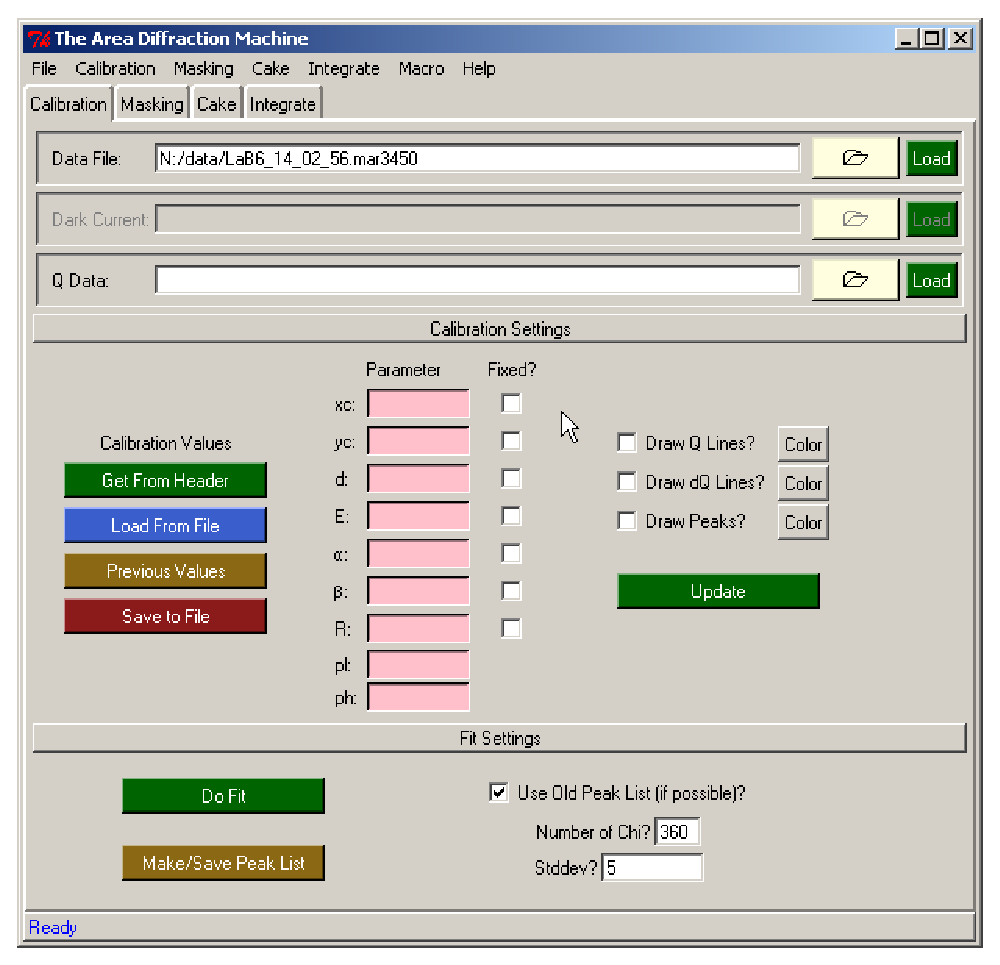
\includegraphics[scale=.75]{figures/calibration_page.eps}

From the \gui{Data File} input, we
load into the program the LaB6 sample file. Once the file
is loaded in, a new window opens up which shows the diffraction
data. This window looks like

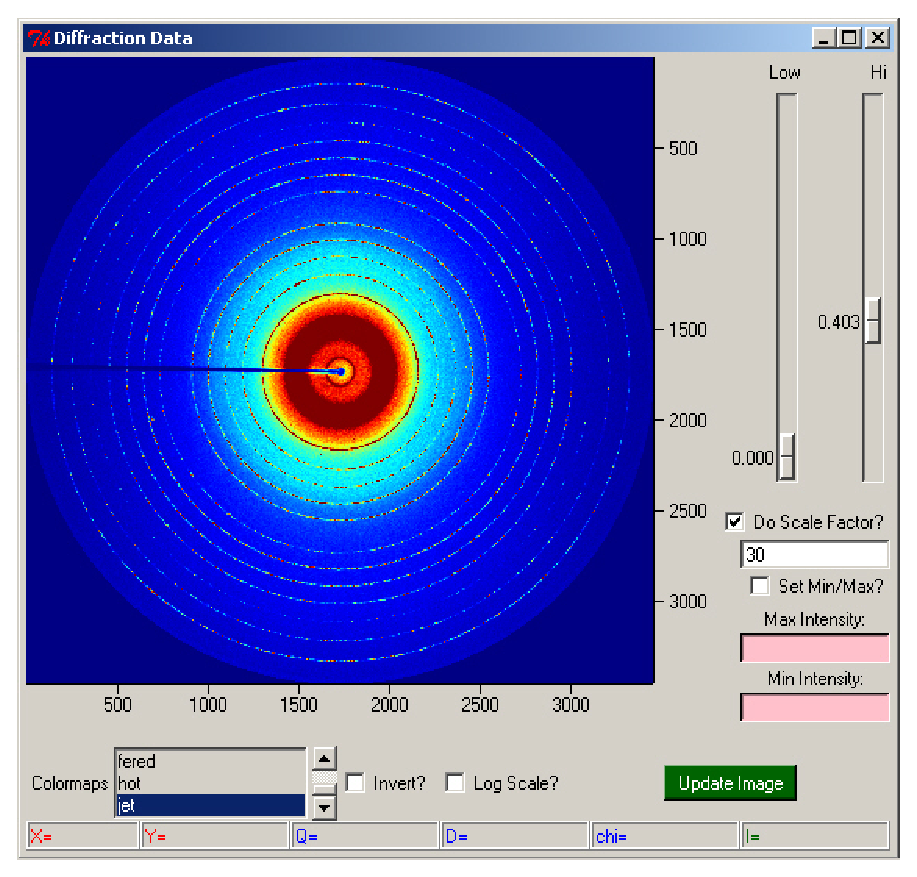
\includegraphics[scale=.75]{figures/diffraction_data_window.eps}

To do the detector calibration, the program must know the 
$Q$ values associated 
with the standard crystal. Since LaB6 is so common, it is
a preset default in the program. We go into the menu bar, 
into the \gui{calibration} menu, into the \gui{Standard Q} menu, 
and then selected Lanthanum Hexaboride. Doing so looks like

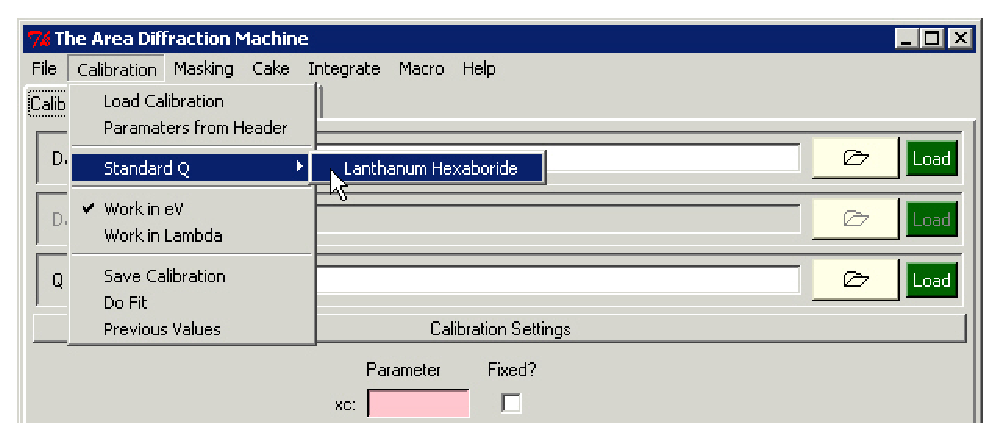
\includegraphics[scale=.75]{figures/standard_q.eps}

(More standard $Q$ files might be added in the future).
In order to perform
image calibration, the program finally needs to know an 
initial guess at the calibration parameters. Although one
could enter these parameters by hand, often times decent
guesses at the experimental parameters are stored in the 
header data inside of the diffraction image. The program
can try to find these header calibration values and put
them into the inputs in the program. To do this, David
pushed the \gui{Get From Header} button. With the image,
the $Q$ values, and an initial guess in the program,
we are ready to do the calibration. 

But first, we want to examine how good the initial guess 
is. To do so, we can select the \gui{Draw Q Lines?}
check box on the Calibration page. When this is selected, 
the program will draw
on top of the diffraction image red lines corresponding
to what diffraction pattern should show up on the
detector (for the given calibration parameters and $Q$
values). For our example, the program displays

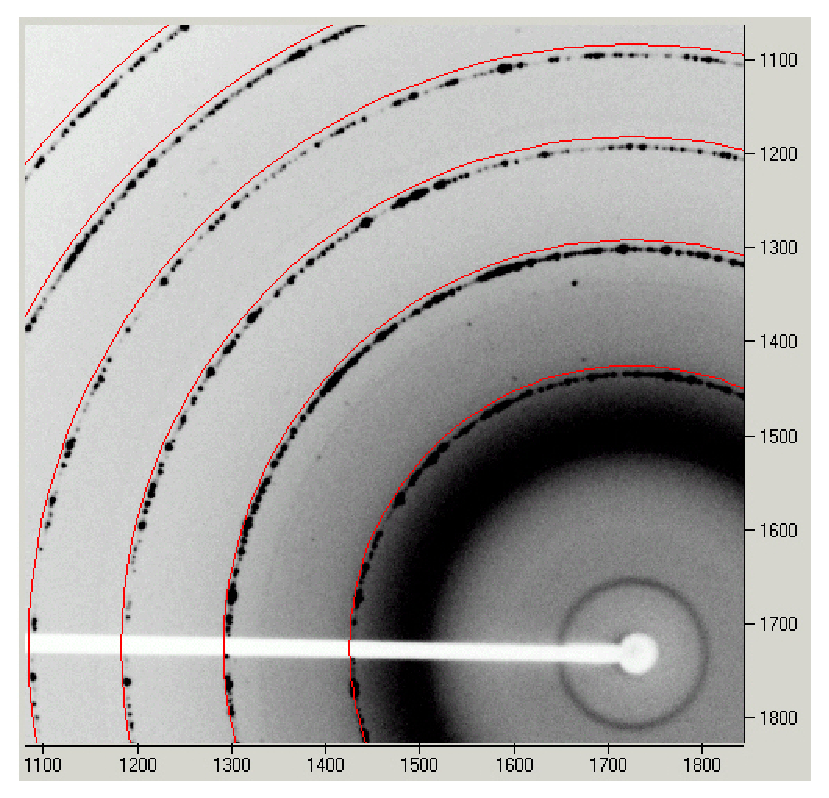
\includegraphics[scale=.75]{figures/bad_calibration_diffraction_image.eps}

Of course, our initial guess isn't
great so the red lines don't match too well with
the loaded patter. The data will look like

We can do an initial cake of the data. A caked plot
is a presentation of the data in a different parameter 
space.  The $x$ axis is $Q$ and the $y$ axis is $\chi$. 
Ideally, if the calibration parameters are known exactly, 
the caked data will show up as many vertical lines. 
We can cake the data by pushing the \gui{AutoCake}
button on the \gui{Cake} page. When we do so, a new cake 
window opens up. For our example, our data looks like

We see that for The caked data with the initial guess 
calibration parameters, our diffraction lines
have a systematic wiggle. It might be hard to see 
with the full image, but by zooming into just one
line, we find the difference to be much more obvious.
This means that our initial guess at 
calibration parameters is not great.

We can now do the calibration. To do so, we push
the \gui{Do Fit} button on the \gui{Calibration}
page. After the calibration finishes, the constant
$Q$ lines drawn on the diffraction image move
so that they are entirely over the diffraction 
pattern. The cake 

This tells us that 


\begin{lstlisting}[caption={'A macro to automate the 
    analysis'}]
Data File:
	C:/Data/
Load From File
    C:/Data/Lab6_cal.dat
Integrate Q Lower?
	0
Integrate Q Upper?
	5
Integrate Number of Q?
	300
Integrate Q-I
Save Integration Data
    PATHNAME/FILENAME_int.dat
\end{lstlisting}



\chapter{Viewing Diffraction Data}
\chapter{Viewing Diffraction Data}\label{viewing_data}

Figure~\ref{calibration_tab} shows the 
Area Diffraction Machine's \gui{Calibration} tab. 
The \gui{Data File:} input can be 
used to load diffraction data either by typing in the filename 
and pushing the load button or by clicking on the folder icon and
using the file selector. After the file is loaded, 
the window shown in figure~\ref{diffraction_data_window}.
will open with the diffraction data in it. 

\begin{SCfigure}[1][bthp]
    \centering
    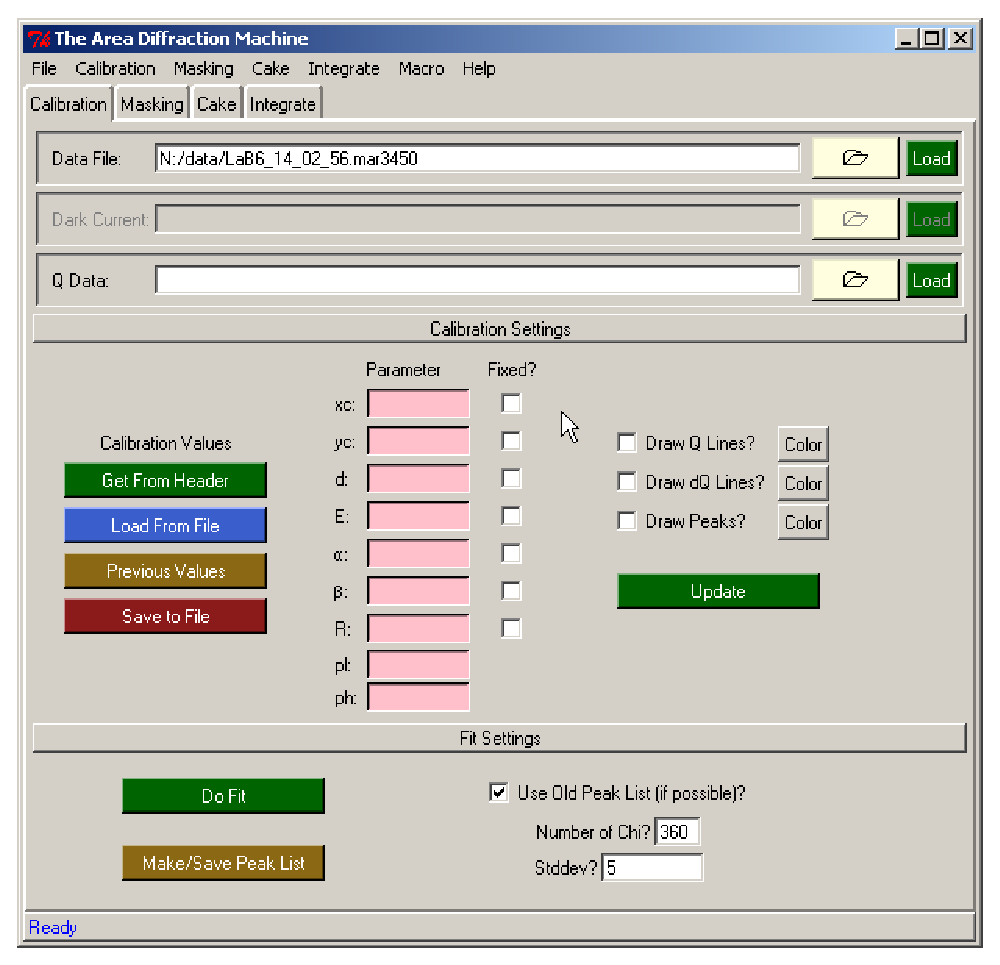
\includegraphics[scale=.75]
    {figures/calibration_tab.eps}
    \caption{The \gui{Calibration} tab. This tab can be used
    to load diffraction data into the program. The 
    \gui{Save Last Fit} button was introduces for version 2 of
    the program.} 
    \label{calibration_tab}
\end{SCfigure}

\begin{SCfigure}[1][bthp]
    \centering
    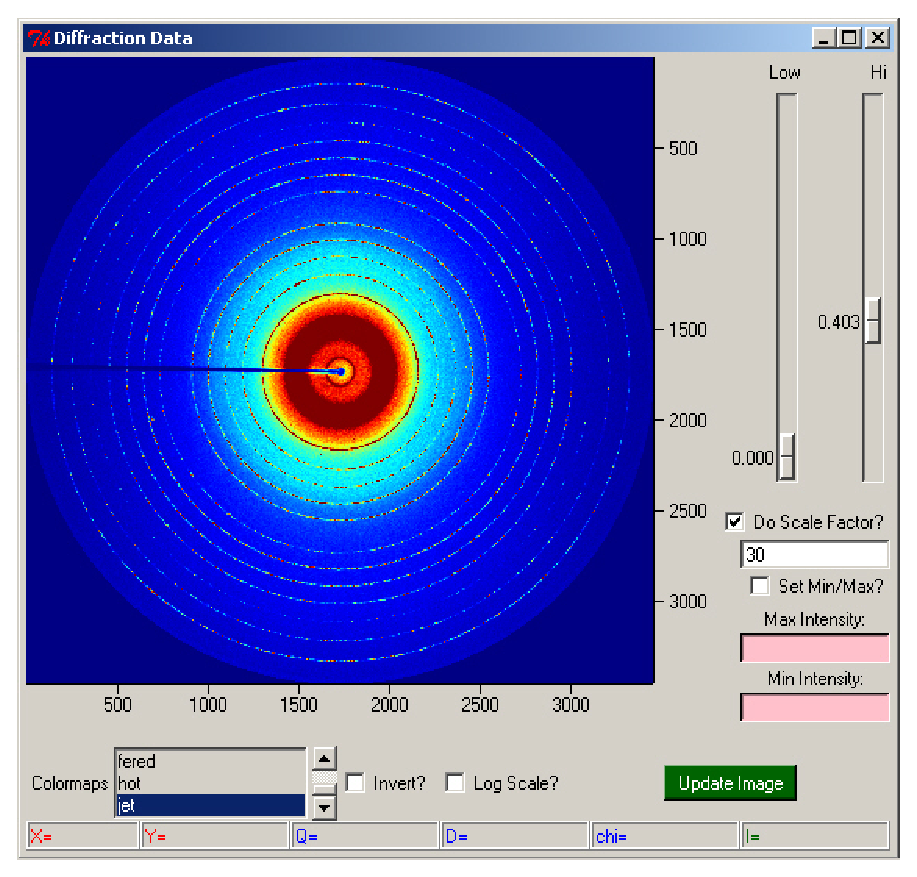
\includegraphics[scale=.75]
    {figures/diffraction_data_window.eps}
    \caption{This diffraction data window will open after 
    a file is loaded.} 
    \label{diffraction_data_window}
\end{SCfigure}

The diffraction data window can be used to interact with 
diffraction data. The window can be used to:
\begin{itemize}
    \item {\em Zoom into the data} -- left click on the data and 
    hold down on the mouse. When moving the mouse around, the
    program will create a resizable square. When the mouse is released,
    the program will zoom into the selected region.
    \item {\em Zoom out of the data} -- right click on
    the data.
    \item {\em Pan across the data} -- hold shift, push down either mouse
    button, and then move the mouse. The image will move 
    with it. Let go of the mouse to stop panning.
    \item {\em Resize the window} -- click on the bottom right corner of
    the window and drag. The window will resize just like any
    other window and the image will become larger or smaller.  
    \item {\em Read coordinates for a selected point} -- when mousing
    over the image, the $x$, $y$, $Q$, $\chi$, and intensity
    values for the current pixel will be displayed at the bottom of the
    window. $Q$ and $\chi$ will only be displayed if valid calibration
    data is loaded into the program. See chapter~\ref{calibration} for
    a discussion of calibration.
    \item {\em Change the Color Map} -- the \gui{Colormaps} selector 
    can be used to change the particular color map used to display the 
    data.
    \item {\em Invert the Color Map} -- The \gui{Invert?} check box can 
    can be used to invert the colors of the color map.
    \item {\em Log Scaling} - By default, intensity values are linearly 
    mapped to colors in the color map. The \gui{Log Scale?} check box 
    can be used to instead apply a log scale mapping of the intensity 
    values to the color map.
    \item {\em Low \& Hi Pixels} -- The sliders to the right of the 
    image can be used to change the intensity scale of the
    image. The low value corresponds to the percentage of
    the most intensity pixel value that is mapped to the lowest part of
    the color map and the hi value corresponds to the percentage of
    the most intense pixel value that is mapped to the highest 
    part of the color map.  This feature is can make more
    visible certain intensity ranges in the image.
    \item {\em ``Do Scale Factor'' and ``Set Min/Max?''} -- Version
    2 of the program introduced the feature \gui{Do Scale Factor?}
    and \gui{Set Min/Max?}. These can be used to override the minimum
    and maximum pixel value used by the Low and Hi sliders. The scale
    factor will simply divide the maximum intensity by this value.
    So if the intensity scale by default goes from 0 to 10000, a
    scale factor of 10 will make the scale instead go from 0 to 1000.
    This feature is especially useful when just a few pixels have
    incredibly large values but the rest have very small values.
    The slides still let you pick a range between 0 and 1000, the
    scale factor simply change what maximum value the slider will
    correspond to. The \gui{Set Min/Max?} option can be used instead
    to set directly the minimum and maximum intensity. To set these
    persistently, use the \gui{Set As Initialization} option described
    in section~\ref{setAsInitializationSection}.
\end{itemize}

\section{File Formats}

The program can load the Mar data \macroline{.mar2300}, 
\macroline{.mar3450}, and the \macroline{.mccd} Mar CCD format
It can load standard \macroline{.tiff} data. 
and the ESRF Data Format \macroline{.edf}.
It can load in Bruker data with extension 
\macroline{.gfrm} and \macroline{.sfrm}.


The program can only deal with square data so whenever non-square
data is loaded, the data will be padded out with blank values
until the data is square.

\section{Clipping High Pixels}

The program stores the diffraction data inside the program as 4 byte integers and 
the largest value that can be stored as an integer is $2^{31}-1 = 2147483647$.
Any intensity values read from diffraction data with value larger then 
this number will be set to this number when stored in the program. In practice, 
this should never be a problem because intensities never range this high.

\section{Loading Multiple Images}

The \gui{Data File:} input can be used to load multiple files
at the same time.
If multiple files are typed into the \gui{Data File:} input and
are separated by spaces, they will all be loaded in. 
Alternately, the diffraction data file 
selector can be used to select and load multiple files.
The program will add the intensities of the images pixel by pixel 
and work with the combined image. The program can only add files 
of the same format.

\section{Saving Diffraction Data}
\index{Save}\index{ESRF Data Format}

Diffraction data can be saved as several popular image formats. 
The data can be saved from the \gui{File} menu using 
the \gui{Save Image} option. The formats currently allowed are \gui{jpg}, 
\gui{gif}, \gui{eps}, \gui{pdf}, \gui{bmp}, \gui{png}, \gui{tiff}, and 
the ESRF data format \gui{edf}.

Images saved as a popular image format will contain whatever
threshold masks, polygon masks, $Q$ lines, $\Delta Q$ lines, and peaks 
are currently displayed and they will be saved
at whatever the current zoom level is.\footnote{This is not the case with 
ESRF data. ESRF data will be saved unzoomed with none
of the lines or masks on top of it.} See chapter~\ref{calibration} for 
a discussion of the $Q$ lines, $\Delta Q$ lines, and peaks. See 
chapter~\ref{pixel_masking} for a discussion of threshold masks and 
polygon masks.

Because the program will pad any non-square data when
it is loaded, the program will always save square
images. If this is undesirable, the saved images
will need to be cropped using another program.

\label{viewing_data}

\chapter{Detector Geometries}
\index{Diffraction Theory}
\index{Detector Geometries}
\begin{SCfigure}
\centering
% Generated with LaTeXDraw 1.9.5
% Sun Apr 20 22:09:06 EDT 2008
% \usepackage[usenames,dvipsnames]{pstricks}
% \usepackage{epsfig}
% \usepackage{pst-grad} % For gradients
% \usepackage{pst-plot} % For axes
\scalebox{1} % Change this value to rescale the drawing.
{
\begin{pspicture}(0,-2.9240625)(6.22,2.9575)
\psellipse[linewidth=0.04,dimen=outer](4.6,0.1825)(1.0,2.0)
\pspolygon[linewidth=0.04,linecolor=white,fillstyle=solid](3.6,1.3559375)(4.2,1.8159375)(4.1,-1.3840625)(3.52,-0.9640625)
\psline[linewidth=0.04cm](2.0,0.1425)(4.64,2.1625)
\psline[linewidth=0.04cm](2.0,0.1425)(4.62,-1.7975)
\psline[linewidth=0.04cm](2.0,0.1425)(5.6,0.1425)
\psline[linewidth=0.04cm](2.0,0.1425)(5.28,-1.2575)
\psline[linewidth=0.04cm](2.0,0.1425)(5.38,1.3425)
\psline[linewidth=0.04cm](0.0,0.1425)(1.6,0.1425)
\psline[linewidth=0.04](3.4,1.2159375)(3.4,2.8825)(6.2,2.0825)(6.2,-2.9175)(3.4,-1.9175)(3.4,-0.9040625)
\usefont{T1}{ptm}{m}{n}
\rput(5.44,2.7825){Detector}
\usefont{T1}{ptm}{m}{n}
\rput(1.69,0.7825){Crystal}
\pspolygon[linewidth=0.04](1.6,0.3025)(1.6,0.0025)(1.8095238,-0.1975)(2.0,-0.0175)(2.0,0.3025)(1.8,0.5025)
\psline[linewidth=0.04cm,linestyle=dashed,dash=0.16cm 0.16cm](3.4,1.2359375)(3.4,-0.9240625)
\psellipse[linewidth=0.04,linestyle=dashed,dash=0.17638889cm 0.10583334cm,dimen=outer](4.6,0.1825)(1.0,2.0)
\end{pspicture} 
}


\caption{An X-Ray diffraction setup. X-rays scatter from a 
3-D sample and are captured by a 2-D detector. In this 
setup, the detector is perpendicular to the incoming 
x-ray beam.}
\label{DiffractionSetup}
\end{SCfigure}

\begin{SCfigure}
\centering
% Generated with LaTeXDraw 1.9.5
% Thu Mar 13 00:25:02 EDT 2008
% \usepackage[usenames,dvipsnames]{pstricks}
% \usepackage{epsfig}
% \usepackage{pst-grad} % For gradients
% \usepackage{pst-plot} % For axes
\scalebox{1} % Change this value to rescale the drawing.
{
\begin{pspicture}(0,-2.92)(6.22,2.92)
\psellipse[linewidth=0.04,dimen=outer](4.6,0.2)(1.0,2.0)
\psline[linewidth=0.04cm](2.0,0.16)(4.64,2.18)
\psline[linewidth=0.04cm](2.0,0.16)(4.62,-1.78)
\psline[linewidth=0.04cm](2.0,0.16)(4.58,0.18)
\psline[linewidth=0.04cm](2.0,0.16)(5.38,1.36)
\psline[linewidth=0.04cm](0.0,0.16)(1.6,0.16)
\psline[linewidth=0.04](3.4,1.7)(3.4,2.9)(6.2,2.1)(6.2,-2.9)(3.4,-1.9)(3.4,-1.3)
\pspolygon[linewidth=0.04](1.6,0.32)(1.6,0.02)(1.8095238,-0.18)(2.0,0.0)(2.0,0.32)(1.8,0.52)
\psline[linewidth=0.04cm](4.56,0.18)(5.38,1.34)
\psline[linewidth=0.04](4.34,0.18)(4.49,0.32)(4.64,0.32)
\psline[linewidth=0.04cm,tbarsize=0.07055555cm 5.0]{|-|}(2.08,-0.22)(4.58,-0.22)
\psline[linewidth=0.04cm,tbarsize=0.07055555cm 5.0]{|-|}(4.9,0.06)(5.7,1.26)
\usefont{T1}{ptm}{m}{n}
\rput(3.2314062,-0.215){\psframebox[linewidth=0.028222222,linecolor=white,fillstyle=solid,framesep=0.0,boxsep=false]{$d$}}
\usefont{T1}{ptm}{m}{n}
\rput(5.2014065,0.585){\psframebox[linewidth=0.02,linecolor=white,fillstyle=solid,framesep=0.02]{$r$}}
\psarc[linewidth=0.04](3.18,0.44){0.38}{315.0}{38.65981}
\usefont{T1}{ptm}{m}{n}
\rput(3.2514062,0.365){$2\theta$}
\pscircle[linewidth=0.04,dimen=outer,fillstyle=solid](5.4,1.36){0.12}
\end{pspicture} 
}


\caption{The same setup as in figure~\ref{DiffractionSetup}. 
Here, $2\theta$ is the scattering angle, $d$ is the distance 
from the crystal to the detector, and $r$ is the distance 
from the center of the detector to some particular point 
(which $2\theta$ is associated with). Note that by center 
of the detector, we mean the point on the detector where 
the beam would hit if did not interact with the crystal.}
\label{MeasureAngleFlatDetector}
\end{SCfigure}

X-ray diffraction is the process of shining a beam of 
high energy x-rays at a regular crystal. This can be 
modeled simply as in figure~\ref{DiffractionSetup}. 
What we have is a series of cones of light that 
emminate preferentially at certain angles normal to 
the outgoing beam. These cones of light are then 
detected by a flat detector, as is shown in the 
diagram. Usually, the interesting thing to measure 
when doing x-ray diffraction are the angles of these 
cones of light. By convention, this angle is called 
$2\theta$. Were the detector to be perfectly perpendicular 
to the incomming beam, as in figure~\ref{DiffractionSetup}, 
our cones of light would be detected as circles of high 
intensity. Were we to know certain experimental parameters 
such as the distance from the sample to the detector and 
the distance from the center of the detecor to a 
particular ring (or really any point on the detector), 
we could easily calculate the scattering angle of light 
that ended up at that particular spot on the detector. 
Suppose that the distance from the crystal to the detector 
is $d$ and the distance from the center of the detector 
to our particular point on the detector is $r$, as is 
shown in figure~\ref{MeasureAngleFlatDetector}. Then the 
scattering angle will be calculated as
\begin{equation}
    \tan2\theta = \frac{r}{d}
\end{equation}
Unfortunnatley, life is not always as simple as this and 
sometimes things get a little bit more complicated. In 
particular, the assumption taht the detector is exactly 
perpendicular to the incomming beam in unphysical. It 
will unphysical because perfect alignment can never be 
acheived and the detector will always in practice be 
slightly offset with respect to the incomming beam, even 
if only slightly. Failing to account for this tilt introduce 
a systematic error in measuring $2\theta$ and doing any other 
sort of data analysis. It is also unphysical because there 
are often good reasons to collect diffraction data from 
detectors at significant tilts . The main reason why this 
is done is to collect data at more extreme angles without 
needing to user larger detectors. This rational is made 
intuitive in figure~\ref{HigherQValues}. So there is a 
need to analyze detectors with tilted geometires. I will 
here present this theory of tilted detectors as it was 
developed by Abhik Kumar in~\cite{Kumar05}.\index{Abhik Kumar}
I could simply refer you to this paper for the results
that I will cite, but this paper is, in my oppinion,
almost absolutely undecipherable. So to save you the
misery of pooring through it yourself, I will do
my best to cleanly work through his findings. 

\begin{SCfigure}
\centering
% Generated with LaTeXDraw 1.9.3
% Wed Aug 08 11:51:23 PDT 2007
% \usepackage[usenames,dvipsnames]{pstricks}
% \usepackage{epsfig}
% \usepackage{pst-grad} % For gradients
% \usepackage{pst-plot} % For axes
\scalebox{1} % Change this value to rescale the drawing.
{
\begin{pspicture}(0,-4.21)(7.5,4.21)
\psline[linewidth=0.04cm](1.32,-1.61)(6.28,1.49)
\psline[linewidth=0.04cm](1.3,-1.65)(7.48,-4.19)
\psline[linewidth=0.04cm](1.28,-1.59)(6.28,-1.59)
\psframe[linewidth=0.04,dimen=outer](1.28,-1.39)(0.88,-1.79)
\psline[linewidth=0.04cm](1.3099908,-1.5937328)(1.9,4.11)
\psline[linewidth=0.04cm](5.26,0.63)(1.28,-1.63)
\psarc[linewidth=0.04](1.96,-1.47){0.66}{347.4712}{45.0}
\psarc[linewidth=0.04](1.09,-1.42){1.09}{351.8699}{70.769325}
\pspolygon[linewidth=0.04](5.28,0.61)(5.28,-2.79)(7.48,-4.19)(7.48,-0.83)
\pspolygon[linewidth=0.04](6.30819,1.5150077)(4.34,4.19)(1.9,4.13)(3.7042418,1.3755335)
\end{pspicture} 
}


\caption{This diagram illustrates how tilted geometries 
allow for the collection of diffraction data at more 
extreme angles without the need for a larger detector.}
\label{HigherQValues}
\end{SCfigure}

What we are interested in is mathematically describing 
position coordinates on a tilted detector by relating 
them to more theoretically motivated quantities such as 
the scattering angles that would lead to a beam hitting
that particular point on the detector. This will be 
the equation that is needed to do the diffraction 
analysis. In order to do this, we must first work
out the transformation of points on a tilted detector
to points on an untilted detector. This is to say
that we want to figure out where on an untilted 
detector the beam would have hit were it to hit
that untilted detector instead of the tilted detector.
We will call the point on the untilted detector
$(x,y)$ as it is measured on the untilted detector
and the point on the tilted detector
$(x''',y''')$ as measured by the tilted detector. 
The notation will become obvious
shortly. This is shown schematically in 
figure~\ref{PhysicalSetup}.


\begin{SCfigure}
\centering
% Generated with LaTeXDraw 1.9.5
% Thu Mar 13 00:56:25 EDT 2008
% \usepackage[usenames,dvipsnames]{pstricks}
% \usepackage{epsfig}
% \usepackage{pst-grad} % For gradients
% \usepackage{pst-plot} % For axes
\scalebox{1} % Change this value to rescale the drawing.
{
\begin{pspicture}(0,-3.14)(8.271875,3.14)
\psline[linewidth=0.04cm,linestyle=dashed,dash=0.17638889cm 0.10583334cm](0.4,0.02)(6.68,2.76)
\psline[linewidth=0.04cm,linestyle=dashed,dash=0.17638889cm 0.10583334cm](0.42,0.02)(3.64,-2.62)
\psline[linewidth=0.04cm,linestyle=dashed,dash=0.17638889cm 0.10583334cm](0.4,0.02)(5.14,0.1)
\psellipse[linewidth=0.04,dimen=outer](5.19,0.0)(0.45,3.14)
\rput{-29.60631}(0.64241344,2.5541434){\psellipse[linewidth=0.04,dimen=outer](5.1536517,0.061624106)(0.27427202,3.115167)}
\psline[linewidth=0.04cm,arrowsize=0.1529cm 2.0,arrowlength=1.4,arrowinset=0.2]{->}(5.16,0.14)(5.12,2.06)
\psline[linewidth=0.04cm,arrowsize=0.1529cm 2.0,arrowlength=1.4,arrowinset=0.2]{->}(5.14,0.1)(6.64,2.62)
\usefont{T1}{ptm}{m}{n}
\rput(3.9714062,2.325){\psframebox[linewidth=0.028222222,linecolor=white,fillstyle=solid,framesep=0.0,boxsep=false]{$(x,y)$}}
\usefont{T1}{ptm}{m}{n}
\rput(7.4714065,2.205){\psframebox[linewidth=0.028222222,linecolor=white,fillstyle=solid,framesep=0.0,boxsep=false]{$(x''',y''')$}}
\psline[linewidth=0.04cm,linestyle=dashed,dash=0.16cm 0.16cm](4.74,-0.14)(5.6,0.36)
\pspolygon[linewidth=0.04](0.0,0.17)(0.0,-0.13)(0.2095238,-0.33)(0.4,-0.15)(0.4,0.17)(0.2,0.37)
\usefont{T1}{ptm}{m}{n}
\rput(5.121406,1.385){\psframebox[linewidth=0.028222222,linecolor=white,fillstyle=solid,framesep=0.0,boxsep=false]{$r$}}
\usefont{T1}{ptm}{m}{n}
\rput(6.1714063,1.485){\psframebox[linewidth=0.028222222,linecolor=white,fillstyle=solid,framesep=0.0,boxsep=false]{$r'''$}}
\end{pspicture} 
}


\caption{The setup of the experiment. Here, the detector 
is titled by some arbitrary angle with respect to the 
incoming beam. We will call some arbitrary point on 
the tilted detector as $(x''',y''')$. We are interested in 
relating this point to the point $(x,y)$ on some imagined 
untilted detector where a scattered beam would have hit 
were that tilted detector set up instead of the tilted
detector.}
\label{PhysicalSetup}
\end{SCfigure}

What we are interested in figuring out is a way of relating 
this point to some other point $(x,y)$ which would be on an 
imagined on a plane perpendicular to the incomming beam 
who's center coincides in 3 dimensional space with the 
center of the tilted detector.

\subsection{The Three Tilt Angels}
\index{$\alpha$}\index{$\beta$}\index{Rotation}
In order to relate these points, we need to find a way to 
describe some arbitrary tilt. To do so, we will need to 
have 3 tilt parameters. We will characterize these tilts 
by two orthogonal rotations about the $x$ and $y$ axis 
and one rotation about the center of the detector. These 
three angles are shown in action in figure~\ref{ThreeTilts}.

\begin{figure}
\centering
\subfloat[The tilt angle $\alpha$.]{
\label{alpha}% Generated with LaTeXDraw 1.9.5
% Sat Apr 26 23:28:53 EDT 2008
% \usepackage[usenames,dvipsnames]{pstricks}
% \usepackage{epsfig}
% \usepackage{pst-grad} % For gradients
% \usepackage{pst-plot} % For axes
\scalebox{1} % Change this value to rescale the drawing.
{
\begin{pspicture}(0,-3.62)(4.82,3.62)
\pspolygon[linewidth=0.04](1.985875,2.2)(4.801875,3.2)(3.217875,-1.8)(0.401875,-3.0)
\usefont{T1}{ptm}{m}{n}
\rput(1.3246872,1.255){$\alpha$}
\pspolygon[linewidth=0.04,linestyle=dashed,dash=0.17638889cm 0.10583334cm](4.481875,-2.2)(1.9514402,-3.6)(0.601875,2.6)(3.13231,3.6)
\psline[linewidth=0.04cm,arrowsize=0.1529cm 2.0,arrowlength=1.4,arrowinset=0.2]{<-cc}(0.201875,-0.62)(4.44,0.56)
\psarc[linewidth=0.04,arrowsize=0.1529cm 2.0,arrowlength=1.4,arrowinset=0.2]{<-cc}(1.2809376,0.9209376){0.79906243}{54.26597}{121.90928}
\usefont{T1}{ptm}{m}{n}
\rput(0.58,-0.135){$\hat x'$}
\pspolygon[linewidth=0.04,linecolor=white,fillstyle=solid](3.66,2.72)(2.84,2.42)(3.78,0.44)(3.9,0.5)(4.1,1.28)
\end{pspicture} 
}

}
\subfloat[The tilt angle $\beta$.]{
\label{beta}% Generated with LaTeXDraw 1.9.5
% Sat Apr 26 23:31:43 EDT 2008
% \usepackage[usenames,dvipsnames]{pstricks}
% \usepackage{epsfig}
% \usepackage{pst-grad} % For gradients
% \usepackage{pst-plot} % For axes
\scalebox{1} % Change this value to rescale the drawing.
{
\begin{pspicture}(0,-3.6375)(3.62,3.6425)
\psline[linewidth=0.04cm,arrowsize=0.1529cm 2.0,arrowlength=1.4,arrowinset=0.2]{<-cc}(1.68,3.6225)(1.86,-3.3375)
\pspolygon[linewidth=0.04,linestyle=dashed,dash=0.17638889cm 0.10583334cm](0.4,2.1775002)(3.6,0.9775002)(3.6,-3.6225)(0.4,-2.4225)
\pspolygon[linewidth=0.04](0.0,1.1775001)(3.2,2.1775002)(3.2,-2.4225)(0.0,-3.6225)
\psarc[linewidth=0.04,arrowsize=0.2cm 2.0,arrowlength=1.4,arrowinset=0.4,fillstyle=solid]{<-cc}(1.62,1.0975003){1.4}{53.414665}{118.39306}
\usefont{T1}{ptm}{m}{n}
\rput(2.321406,2.8625){$\beta$}
\usefont{T1}{ptm}{m}{n}
\rput(1.29,3.3625){$\hat{y}$}
\pspolygon[linewidth=0.04,linecolor=white,fillstyle=solid](1.78,1.6825)(3.1188407,2.0825)(3.16,1.1425)(2.0692754,1.1825)
\end{pspicture} 
}

}
\subfloat[The rotation angle $R$.]{
\label{R}% Generated with LaTeXDraw 1.9.5
% Fri Apr 04 00:00:58 EDT 2008
% \usepackage[usenames,dvipsnames]{pstricks}
% \usepackage{epsfig}
% \usepackage{pst-grad} % For gradients
% \usepackage{pst-plot} % For axes
\scalebox{1} % Change this value to rescale the drawing.
{
\begin{pspicture}(0,-3.0736678)(5.98,3.0736675)
\psframe[linewidth=0.04,linestyle=dashed,dash=0.16cm 0.16cm,dimen=outer](3.9,2.8)(1.3,-2.7)
\rput{-27.108658}(0.2746401,1.1391985){\psframe[linewidth=0.04,dimen=outer](3.9051368,2.7414577)(1.094863,-2.7414577)}
\psline[linewidth=0.04cm,linestyle=dashed,dash=0.16cm 0.16cm](2.6,2.8)(2.7,-2.7)
\psline[linewidth=0.04cm](3.8,2.4)(1.2,-2.4)
\psarc[linewidth=0.04,arrowsize=0.1529cm 2.0,arrowlength=1.4,arrowinset=0.2]{<-}(2.6762128,1.1548789){0.79}{30.963757}{91.39718}
\usefont{T1}{ptm}{m}{n}
\rput(2.927619,1.4098788){$R$}
\psline[linewidth=0.04,linestyle=dashed,dash=0.16cm 0.16cm,arrowsize=0.1529cm 2.0,arrowlength=1.4,arrowinset=0.2]{<->}(4.2000003,-0.9)(4.250769,-1.9799999)(5.3,-1.9491428)
\usefont{T1}{ptm}{m}{n}
\rput(5.06,-0.895){$\hat{y}''$}
\usefont{T1}{ptm}{m}{n}
\rput(5.16,-1.595){$\hat{x}''$}
\end{pspicture} 
}

}
\caption{Any detector rotation can be characterized 
as a rotation by both $\alpha$ and $\beta$.}
\label{ThreeTilts}
\end{figure}

In order to find this relationship, we will apply each of these 
rotations separately, one after another. And the combination 
of each of the three rotations will yield the total 
transformation.


\subsection{The $R$ Rotation}

\begin{SCfigure}
\centering
% Generated with LaTeXDraw 1.9.5
% Sat Apr 19 15:30:16 EDT 2008
% \usepackage[usenames,dvipsnames]{pstricks}
% \usepackage{epsfig}
% \usepackage{pst-grad} % For gradients
% \usepackage{pst-plot} % For axes
\scalebox{1} % Change this value to rescale the drawing.
{
\begin{pspicture}(0,-2.575)(9.741406,2.555)
\pspolygon[linewidth=0.04](0.38,-0.355)(7.18,-0.415)(5.24,-2.465)
\psline[linewidth=0.04](0.36,-0.355)(9.42,2.535)(8.26,-0.245)
\psline[linewidth=0.04,linestyle=dashed,dash=0.16cm 0.16cm,arrowsize=0.1529cm 2.0,arrowlength=1.4,arrowinset=0.2]{<->}(8.4,-0.845)(7.92,-1.915)(6.88,-2.425)
\usefont{T1}{ptm}{m}{n}
\rput(8.621407,-1.53){$\hat{y}''$}
\usefont{T1}{ptm}{m}{n}
\rput(7.6714063,-2.35){$\hat{x}''$}
\pspolygon[linewidth=0.04,fillstyle=solid](0.0,-0.175)(0.0,-0.475)(0.2095238,-0.675)(0.4,-0.495)(0.4,-0.175)(0.2,0.025)
\pspolygon[linewidth=0.04,fillstyle=solid](5.3,-2.405)(7.36,1.215)(9.42,2.515)(8.36,-0.305)
\usefont{T1}{ptm}{m}{n}
\rput(8.171407,0.99){\psframebox[linewidth=0.028222222,linecolor=white,fillstyle=solid,framesep=0.0,boxsep=false]{$(x''',y''')$}}
\psellipse[linewidth=0.04,dimen=outer,fillstyle=solid](8.18,0.155)(0.12,0.11)
\psellipse[linewidth=0.04,dimen=outer,fillstyle=solid](7.42,0.495)(0.12,0.11)
\psline[linewidth=0.04cm,arrowsize=0.1529cm 2.0,arrowlength=1.4,arrowinset=0.2]{->}(5.36,-2.345)(7.34,0.345)
\usefont{T1}{ptm}{m}{n}
\rput(9.051406,0.29){\psframebox[linewidth=0.028222222,linecolor=white,fillstyle=solid,framesep=0.0,boxsep=false]{$(x'',y'')$}}
\psline[linewidth=0.04cm,arrowsize=0.1529cm 2.0,arrowlength=1.4,arrowinset=0.2]{->}(5.32,-2.385)(8.04,-0.015)
\psarc[linewidth=0.04,arrowsize=0.1cm 2.0,arrowlength=1.4,arrowinset=0.2]{->}(6.78,-1.075){0.84}{38.65981}{79.28688}
\usefont{T1}{ptm}{m}{n}
\rput(6.6814065,-0.89){$R$}
\end{pspicture} 
}


\caption{This figure shows how points on a detector rotated 
by angle $R$ relate to the unrotated points. Remember that
a rotation of the plane is equivalent to the rotation of the
coordinates on the plane (which is what I have drawn).}
\label{RotationFormula}
\end{SCfigure}

We will first deal with the physical rotation by angle $R$ 
of the plane. What we have to deal with is the point $(x,y)$
on a plane being superimposed onto the point $(x',y')$ on 
another plane which is rotated by an angle $R$. This is shown
schematically in figure~\ref{RotationFormula}. The rotation of
the plane is mathematically equivalent to rotating the coordinates
and the equation describing the rotation of a plane is:
\begin{eqnarray}
    x&=&x'\cos R + y'cos R\\
    y&=&y'\cos R - x'cos R
\end{eqnarray}

\subsection{The $\beta$ Tilt}

\begin{figure}
\centering
\subfloat[]{\label{PitchX_A}% Generated with LaTeXDraw 1.9.5
% Tue Feb 12 22:42:23 EST 2008
% \usepackage[usenames,dvipsnames]{pstricks}
% \usepackage{epsfig}
% \usepackage{pst-grad} % For gradients
% \usepackage{pst-plot} % For axes
\scalebox{1} % Change this value to rescale the drawing.
{
\begin{pspicture}(0,-2.4992187)(7.401875,2.5192187)
\pspolygon[linewidth=0.04](0.48,-0.43921876)(7.24,-0.45921874)(5.34,-2.4792187)
\psline[linewidth=0.04](0.42,-0.39921874)(7.2,1.8007812)(7.26,-0.41921875)
\pspolygon[linewidth=0.04](0.0,-0.25921875)(0.0,-0.55921876)(0.2095238,-0.75921875)(0.4,-0.57921875)(0.4,-0.25921875)(0.2,-0.05921875)
\pspolygon[linewidth=0.04,fillstyle=solid](3.92,-1.8192188)(3.98,-0.022702621)(5.42,1.2407813)(5.42,-0.41000822)
\pspolygon[linewidth=0.04,fillstyle=solid](3.92,-1.8592187)(3.96,-0.03921875)(7.18,1.8007812)(7.22,-0.39921874)
\psellipse[linewidth=0.04,dimen=outer,fillstyle=solid](5.38,1.2107812)(0.12,0.11)
\psellipse[linewidth=0.04,dimen=outer,fillstyle=solid](7.14,1.7707813)(0.12,0.11)
\psline[linewidth=0.04](5.0,-2.3592188)(5.26,-2.0792189)(5.58,-2.2192187)
\psarc[linewidth=0.04,arrowsize=0.1cm 2.0,arrowlength=1.4,arrowinset=0.2]{<-}(4.9,0.32078126){0.66}{42.70939}{73.61046}
\usefont{T1}{ptm}{m}{n}
\rput(4.5314064,0.61078125){$\beta$}
\psline[linewidth=0.04,linestyle=dashed,dash=0.16cm 0.16cm,arrowsize=0.1529cm 2.0,arrowlength=1.4,arrowinset=0.2]{<->}(1.62,2.2807813)(1.62,1.2207812)(0.82,0.56078124)
\usefont{T1}{ptm}{m}{n}
\rput(1.9614062,1.9107813){$\hat{y}$}
\usefont{T1}{ptm}{m}{n}
\rput(1.6314063,0.85078126){$\hat{x}$}
\usefont{T1}{ptm}{m}{n}
\rput(5.581406,1.7907813){$(x,y)$}
\usefont{T1}{ptm}{m}{n}
\rput(6.7614064,2.3307812){$(x',y')$}
\psline[linewidth=0.04cm,linestyle=dashed,dash=0.16cm 0.16cm](3.94,-0.43921876)(7.22,-0.39921874)
\psline[linewidth=0.04cm,linestyle=dashed,dash=0.16cm 0.16cm](5.4,0.7607812)(5.4,-0.37921876)
\end{pspicture} 
}

} 
\hfill
\subfloat[]{
\label{PitchX_B}% Generated with LaTeXDraw 1.9.5
% Thu Mar 13 00:19:09 EDT 2008
% \usepackage[usenames,dvipsnames]{pstricks}
% \usepackage{epsfig}
% \usepackage{pst-grad} % For gradients
% \usepackage{pst-plot} % For axes
\scalebox{1} % Change this value to rescale the drawing.
{
\begin{pspicture}(0,-2.23)(6.818594,2.21)
\usefont{T1}{ptm}{m}{n}
\rput{1.3976438}(-0.0020833788,-0.075975105){\rput(3.0943067,-0.12885925){$x$}}
\usefont{T1}{ptm}{m}{n}
\rput{-1.0330194}(0.014848421,0.083165735){\rput(4.600972,-0.787422){$x'$}}
\pspolygon[linewidth=0.04](0.18,1.05)(6.06,-0.37)(3.82,-1.99)
\psline[linewidth=0.04cm,tbarsize=0.07055555cm 5.0]{|-|}(0.0,0.67)(2.2,-1.15)
\psline[linewidth=0.04cm,tbarsize=0.07055555cm 5.0]{|-|}(3.5,-2.17)(2.3,-1.21)
\psline[linewidth=0.04cm,tbarsize=0.07055555cm 5.0]{|-|}(4.0,-2.21)(6.26,-0.55)
\usefont{T1}{ptm}{m}{n}
\rput{-358.90466}(-0.031908773,-0.1122255){\rput(5.8351817,-1.7306391){\psframebox*[framesep=0, boxsep=false,fillcolor=white] {$x'\cos\beta$}}}
\usefont{T1}{ptm}{m}{n}
\rput{-0.92512906}(0.03058399,0.03998597){\rput(2.4726164,-1.879585){\psframebox*[framesep=0, boxsep=false,fillcolor=white] {$x'\sin\beta$}}}
\usefont{T1}{ptm}{m}{n}
\rput{0.0600076}(-0,-0.0012422148){\rput(1.1668588,-0.30427834){\psframebox*[framesep=0, boxsep=false,fillcolor=white] {$d$}}}
\psline[linewidth=0.04cm](3.881024,0.15001266)(3.86,1.73)
\usefont{T1}{ptm}{m}{n}
\rput(3.5514061,1.18){$y$}
\psline[linewidth=0.04](3.92,0.67)(3.62,0.39)(3.64,-0.01)
\usefont{T1}{ptm}{m}{n}
\rput(5.6714063,1.32){$y'$}
\psline[linewidth=0.04](0.32,1.07)(6.0,2.09)(6.08,-0.37)
\psarc[linewidth=0.04,arrowsize=0.1529cm 2.0,arrowlength=1.4,arrowinset=0.2]{<-}(3.51,-0.8){0.75}{24.443954}{82.874985}
\usefont{T1}{ptm}{m}{n}
\rput(3.5514061,-0.56){$\beta$}
\psline[linewidth=0.04](2.26,-0.67)(2.54,-0.45)(2.82,-0.67)
\psline[linewidth=0.04](3.56,-1.81)(3.8624,-1.57)(4.1,-1.77)
\pspolygon[linewidth=0.04,fillstyle=solid](0.1,1.23)(0.1,0.93)(0.26761904,0.73)(0.42,0.91)(0.42,1.23)(0.26,1.43)
\psellipse[linewidth=0.04,dimen=outer,fillstyle=solid](3.86,1.72)(0.12,0.11)
\psellipse[linewidth=0.04,dimen=outer,fillstyle=solid](5.98,2.1)(0.12,0.11)
\psline[linewidth=0.04](3.88,0.17)(2.56,-0.87)(6.1,-0.35)
\psline[linewidth=0.04](6.06,0.09)(5.76,-0.19)(5.78,-0.59)
\usefont{T1}{ptm}{m}{n}
\rput(2.5214062,0.5){\psframebox*[framesep=0, boxsep=false,fillcolor=white] {$a$}}
\usefont{T1}{ptm}{m}{n}
\rput(4.871406,-0.02){\psframebox*[framesep=0, boxsep=false,fillcolor=white] {$b$}}
\end{pspicture} 
}

}
\caption{A diagram of the situation depicted in 
figure~\ref{PhysicalSetup} where only the 
$\beta$ rotation has been applied.}
\label{PitchX}
\end{figure}

We will now take the point $(x',y')$ and on the rotated plane 
and see what the coordinates of the corresponding point
$(x'',y'')$ would be if the point was projected onto another
plane titled by an angle $\beta$ around $\hat{y}$.
This is to say that we will figure out where on the tilted
plane a beam would hit were it not to hit that detector 
instead of the un-tilted detector.
This relationship is diagrammed in figure~\ref{PitchX}.  
We can use the geometry of these diagrams to figure out
the relationships between these coordinates. Using
the property of similar triangles, we see that
\begin{equation}
    \frac{x'}{d}=\frac{x''\cos\beta}{d+x''\sin\beta}.
\end{equation}
From this it follows that 
\begin{equation}\label{xTermsxPrime}
    \boxed{x' = \frac{dx''\cos\beta}{d+x''\sin\beta}.}
\end{equation}
Using similar triangles again, we see that
\begin{eqnarray}
    \frac{y'}{a}&=&\frac{y''}{a+b}\\
    \frac{d}{a}&=&\frac{d+x''\sin\beta}{a+b}.
\end{eqnarray}
from which it follows that
\begin{equation}\label{yTermsxPrime}
	\boxed{y'= \frac{dy''}{d+x''\sin\beta}.}
\end{equation}
So, equation~\ref{xTermsxPrime} and \ref{yTermsxPrime} give us 
the proper geometrical equations for relating a point on the 
un-tilted plane $(x',y')$ to the corresponding point 
$(x'',y'')$ on the tilted plane.


\subsection{The $\alpha$ Roll}
We can now take this point $(x'',y'')$ on the tilted 
plane and project it onto another plane which has both 
a tilt and roll by an angle $\alpha$ around $\hat{x}$ 
applied to it. This is to say that we can determine 
where beam that hit a point on the tilted detector 
would have hit were it to instead hit a tilted and 
rolled detector. This is shown schematically in 
figure~\ref{PitchY_A}. A more geometric view of 
the situation can be seen in figure~\ref{PitchY_B} and 
a cross section of the $x$
axis of this figure can be seen in figure~\ref{PitchY_C}.

\begin{SCfigure}
\centering
% Generated with LaTeXDraw 1.9.5
% Tue Feb 05 04:35:09 EST 2008
% \usepackage[usenames,dvipsnames]{pstricks}
% \usepackage{epsfig}
% \usepackage{pst-grad} % For gradients
% \usepackage{pst-plot} % For axes
\scalebox{1} % Change this value to rescale the drawing.
{
\begin{pspicture}(0,-3.91)(10.94,3.91)
\pspolygon[linewidth=0.04](0.24,0.95)(9.62,-1.3107895)(6.0466666,-3.89)
\usefont{T1}{ptm}{m}{n}
\rput(5.68,1.215){$y'$}
\psline[linewidth=0.04](0.26,0.97)(6.06,1.99)(6.14,-0.47)
\pspolygon[linewidth=0.04,fillstyle=solid](0.0,1.11)(0.0,0.81)(0.16761903,0.61)(0.32,0.79)(0.32,1.11)(0.16,1.31)
\psline[linewidth=0.04](9.66,-1.31)(9.82,2.59)(6.1,1.99)
\usefont{T1}{ptm}{m}{n}
\rput(6.21,3.195){$(x'',y'')$}
\usefont{T1}{ptm}{m}{n}
\rput(10.19,3.175){$(x''',y''')$}
\psellipse[linewidth=0.04,dimen=outer,fillstyle=solid](9.8,2.58)(0.12,0.11)
\pspolygon[linewidth=0.04,fillstyle=solid](2.62,-0.99)(6.1,-0.45)(6.06,1.97)(2.54,1.71)
\pspolygon[linewidth=0.04,fillstyle=solid](2.62,-1.01)(6.08,-0.45)(9.8,2.61)(4.54,2.19)
\psline[linewidth=0.04cm,arrowsize=0.1529cm 2.0,arrowlength=1.4,arrowinset=0.2]{->}(5.94,2.93)(5.94,2.43)
\usefont{T1}{ptm}{m}{n}
\rput(2.86,0.155){$\alpha$}
\psarc[linewidth=0.04,arrowsize=0.1529cm 2.0,arrowlength=1.4,arrowinset=0.2]{<-}(2.49,-0.26){0.97}{38.08877}{86.63354}
\psline[linewidth=0.04cm,linestyle=dashed,dash=0.16cm 0.16cm](6.16,-0.39)(8.7,2.77)
\psline[linewidth=0.04cm,linestyle=dashed,dash=0.16cm 0.16cm](8.78,2.81)(9.78,2.67)
\psline[linewidth=0.04cm](6.1,-0.41)(8.44,-2.07)
\psline[linewidth=0.04cm,linestyle=dashed,dash=0.16cm 0.16cm](8.46,-2.13)(8.74,2.77)
\psline[linewidth=0.04,linestyle=dashed,dash=0.16cm 0.16cm,arrowsize=0.1529cm 2.0,arrowlength=1.4,arrowinset=0.2]{<->}(2.7,3.89)(2.7,2.61)(1.54,2.13)
\usefont{T1}{ptm}{m}{n}
\rput(3.12,3.395){$\hat{y}$}
\usefont{T1}{ptm}{m}{n}
\rput(2.58,2.215){$\hat{x}$}
\end{pspicture} 
}

 
\label{PitchY_A}
\caption{In this figure, we see a tilted detector 
and then a detector which is both tilted and rolled
by an angle $\alpha$ around $\hat{x}$.}
\end{SCfigure}

\begin{SCfigure}
\centering
% Generated with LaTeXDraw 1.9.5
% Sat Apr 19 15:16:46 EDT 2008
% \usepackage[usenames,dvipsnames]{pstricks}
% \usepackage{epsfig}
% \usepackage{pst-grad} % For gradients
% \usepackage{pst-plot} % For axes
\scalebox{1} % Change this value to rescale the drawing.
{
\begin{pspicture}(0,-3.26)(9.16,3.28)
\usefont{T1}{ptm}{m}{n}
\rput{1.3976438}(0.0039254855,-0.07954958){\rput(3.2429004,0.11614075){$x$}}
\usefont{T1}{ptm}{m}{n}
\rput{-1.0330194}(0.011214565,0.08913997){\rput(4.929566,-0.58242196){$x''$}}
\pspolygon[linewidth=0.04](0.32,1.3)(6.2,-0.12)(4.06,-1.84)
\psline[linewidth=0.04cm,tbarsize=0.07055555cm 5.0]{|-|}(0.26,0.92)(2.34,-0.9)
\psline[linewidth=0.04cm,tbarsize=0.07055555cm 5.0]{|-|}(4.44,-2.58)(2.44,-0.96)
\usefont{T1}{ptm}{m}{n}
\rput{-0.92512906}(0.024716513,0.042286336){\rput(2.61121,-1.514585){\psframebox*[framesep=0, boxsep=false,fillcolor=white] {$x''\sin\beta$}}}
\usefont{T1}{ptm}{m}{n}
\rput{0.0600076}(-0,-0.0013253981){\rput(1.2454526,-0.09927834){\psframebox*[framesep=0, boxsep=false,fillcolor=white] {$d$}}}
\psline[linewidth=0.04cm](4.0210238,0.40001267)(4.0,1.98)
\usefont{T1}{ptm}{m}{n}
\rput(3.67,1.305){$y$}
\psline[linewidth=0.04](4.06,0.92)(3.76,0.64)(3.78,0.24)
\psline[linewidth=0.04](0.32,1.3)(6.14,2.34)(6.22,-0.12)
\psarc[linewidth=0.04,arrowsize=0.1529cm 2.0,arrowlength=1.4,arrowinset=0.2]{<-}(3.27,-0.53){0.75}{10.713123}{59.036243}
\usefont{T1}{ptm}{m}{n}
\rput(3.51,-0.295){$\beta$}
\psline[linewidth=0.04](3.8,-1.64)(4.1024,-1.4)(4.34,-1.62)
\pspolygon[linewidth=0.04,fillstyle=solid](0.0,1.46)(0.0,1.16)(0.16761903,0.96)(0.32,1.14)(0.32,1.46)(0.16,1.66)
\psline[linewidth=0.04](4.02,0.42)(2.7,-0.62)(6.24,-0.1)
\psline[linewidth=0.04](6.2,0.34)(5.9,0.06)(5.92,-0.34)
\usefont{T1}{ptm}{m}{n}
\rput(2.4,0.825){\psframebox*[framesep=0, boxsep=false,fillcolor=white] {$a$}}
\psline[linewidth=0.04cm](4.02,1.96)(8.16,2.7)
\psellipse[linewidth=0.04,dimen=outer,fillstyle=solid](4.0,1.97)(0.12,0.11)
\psline[linewidth=0.04cm](0.58,1.08)(5.5,-3.04)
\psline[linewidth=0.04cm](2.62,-0.62)(7.84,0.14)
\psline[linewidth=0.04cm](3.98,0.42)(8.16,-0.6)
\usefont{T1}{ptm}{m}{n}
\rput(4.85,0.185){\psframebox*[framesep=0, boxsep=false,fillcolor=white] {$b$}}
\psline[linewidth=0.04cm](7.82,0.16)(8.18,2.72)
\psline[linewidth=0.04cm](8.18,2.7)(8.18,-0.56)
\psline[linewidth=0.04cm,linestyle=dashed,dash=0.16cm 0.16cm](7.74,1.18)(7.8,0.16)
\usefont{T1}{ptm}{m}{n}
\rput(7.6,0.665){$\alpha$}
\usefont{T1}{ptm}{m}{n}
\rput(7.86,2.145){$\alpha$}
\psline[linewidth=0.04cm,linestyle=dashed,dash=0.16cm 0.16cm](7.82,0.12)(4.74,-2.38)
\psline[linewidth=0.04cm](8.18,-0.56)(7.82,0.14)
\psline[linewidth=0.04cm,tbarsize=0.07055555cm 5.0]{|-|}(8.48,-0.54)(8.46,2.6)
\psellipse[linewidth=0.04,dimen=outer,fillstyle=solid](6.14,2.35)(0.12,0.11)
\psellipse[linewidth=0.04,dimen=outer,fillstyle=solid](8.18,2.71)(0.12,0.11)
\usefont{T1}{ptm}{m}{n}
\rput(4.11,2.345){$(x,y)$}
\usefont{T1}{ptm}{m}{n}
\rput(6.17,2.745){$(x',y')$}
\usefont{T1}{ptm}{m}{n}
\rput(8.31,3.085){$(x'',y'')$}
\usefont{T1}{ptm}{m}{n}
\rput(8.85,1.445){$h$}
\psline[linewidth=0.04cm](8.18,-0.56)(5.5,-3.04)
\usefont{T1}{ptm}{m}{n}
\rput(7.0,0.285){$e$}
\psline[linewidth=0.04cm,tbarsize=0.07055555cm 5.0]{|-|}(5.68,-3.22)(8.32,-0.74)
\usefont{T1}{ptm}{m}{n}
\rput(7.37,-1.955){\psframebox*[framesep=0, boxsep=false,fillcolor=white] {$l$}}
\psline[linewidth=0.04](5.22,-2.82)(5.5224,-2.58)(5.76,-2.8)
\usefont{T1}{ptm}{m}{n}
\rput{-1.0330194}(-0.026544517,0.1406858){\rput(7.769566,1.557578){$y''$}}
\usefont{T1}{ptm}{m}{n}
\rput{-1.0330194}(-0.021456113,0.10512067){\rput(5.799566,1.257578){$y'$}}
\psline[linewidth=0.04cm,tbarsize=0.07055555cm 5.0]{|-|}(5.28,-3.24)(4.52,-2.62)
\usefont{T1}{ptm}{m}{n}
\rput(4.84,-2.935){\psframebox*[framesep=0, boxsep=false,fillcolor=white] {$f$}}
\usefont{T1}{ptm}{m}{n}
\rput(6.9,-0.275){\psframebox*[framesep=0, boxsep=false,fillcolor=white] {$c$}}
\psarc[linewidth=0.04](8.19,1.73){0.25}{225.0}{273.8141}
\rput{-180.0}(15.54,1.7){\psarc[linewidth=0.04](7.77,0.85){0.25}{225.0}{273.8141}}
\end{pspicture} 
}

 
\label{PitchY_B}
\end{SCfigure}

\begin{SCfigure}
\centering
% Generated with LaTeXDraw 1.9.5
% Tue Feb 05 05:23:41 EST 2008
% \usepackage[usenames,dvipsnames]{pstricks}
% \usepackage{epsfig}
% \usepackage{pst-grad} % For gradients
% \usepackage{pst-plot} % For axes
\scalebox{1} % Change this value to rescale the drawing.
{
\begin{pspicture}(0,-3.94)(11.148838,3.92)
\pspolygon[linewidth=0.04](0.26913854,-2.5818686)(8.749122,-2.5195673)(8.788253,1.7014359)
\psline[linewidth=0.04cm](3.9488378,-2.54)(3.9488378,-0.68)
\psline[linewidth=0.04cm](5.6888375,1.7)(5.6488376,-2.5)
\psline[linewidth=0.04cm](3.9488378,-2.5)(5.6688375,0.16)
\psline[linewidth=0.04cm](5.6688375,0.14)(8.748837,0.18)
\psline[linewidth=0.04cm](5.6688375,1.7)(8.748837,1.72)
\usefont{T1}{ptm}{m}{n}
\rput(7.2488375,0.925){\psframebox*[framesep=0, boxsep=false,fillcolor=white] {$c$}}
\usefont{T1}{ptm}{m}{n}
\rput(4.9188375,-0.195){\psframebox*[framesep=0, boxsep=false,fillcolor=white] {$b$}}
\usefont{T1}{ptm}{m}{n}
\rput(2.3088377,-1.495){\psframebox*[framesep=0, boxsep=false,fillcolor=white] {$a$}}
\usefont{T1}{ptm}{m}{n}
\rput(3.9288378,-1.675){\psframebox*[framesep=0, boxsep=false,fillcolor=white] {$x'$}}
\usefont{T1}{ptm}{m}{n}
\rput(5.058838,-1.095){\psframebox*[framesep=0, boxsep=false,fillcolor=white] {$x''$}}
\psline[linewidth=0.04cm](5.6888375,1.72)(3.0288377,-2.54)
\psline[linewidth=0.04cm](8.748837,1.74)(6.0888376,-2.52)
\usefont{T1}{ptm}{m}{n}
\rput(5.0488377,0.545){\psframebox*[framesep=0, boxsep=false,fillcolor=white] {$x'''$}}
\usefont{T1}{ptm}{m}{n}
\rput(7.2688375,-0.755){\psframebox*[framesep=0, boxsep=false,fillcolor=white] {$x'''$}}
\pspolygon[linewidth=0.04,fillstyle=solid](0.004397999,-2.4366233)(0.0,-2.736591)(0.16466902,-2.9390268)(0.3196724,-2.76128)(0.32436362,-2.4413145)(0.1673128,-2.2389905)
\psline[linewidth=0.04cm,tbarsize=0.07055555cm 5.0]{|-|}(0.26883766,-3.38)(3.8888376,-3.38)
\psline[linewidth=0.04cm,tbarsize=0.07055555cm 5.0]{|-|}(3.0088377,-3.02)(5.868838,-3.0)
\psline[linewidth=0.04cm,tbarsize=0.07055555cm 5.0]{|-|}(6.1488376,-3.0)(8.728838,-3.02)
\usefont{T1}{ptm}{m}{n}
\rput(2.1788378,-3.395){\psframebox*[framesep=0, boxsep=false,fillcolor=white] {$d$}}
\usefont{T1}{ptm}{m}{n}
\rput(4.5088377,-2.975){\psframebox*[framesep=0, boxsep=false,fillcolor=white] {$y'''\sin\alpha$}}
\usefont{T1}{ptm}{m}{n}
\rput(7.1088376,0.145){\psframebox*[framesep=0, boxsep=false,fillcolor=white] {$y'''\sin\alpha$}}
\usefont{T1}{ptm}{m}{n}
\rput(7.1088376,1.785){\psframebox*[framesep=0, boxsep=false,fillcolor=white] {$y'''\sin\alpha$}}
\usefont{T1}{ptm}{m}{n}
\rput(7.3188376,-3.015){\psframebox*[framesep=0, boxsep=false,fillcolor=white] {$x'''\sin\beta$}}
\psline[linewidth=0.04cm,tbarsize=0.07055555cm 5.0]{|-|}(9.168838,1.76)(9.168838,-2.46)
\usefont{T1}{ptm}{m}{n}
\rput(10.018838,-0.395){\psframebox*[framesep=0, boxsep=false,fillcolor=white] {$x'''\cos\alpha$}}
\psline[linewidth=0.04cm,tbarsize=0.07055555cm 5.0]{|-|}(2.9288378,-3.74)(3.8688376,-3.74)
\usefont{T1}{ptm}{m}{n}
\rput(3.3588376,-3.755){\psframebox*[framesep=0, boxsep=false,fillcolor=white] {$o$}}
\psline[linewidth=0.04cm,linestyle=dashed,dash=0.16cm 0.16cm](2.9688377,-2.54)(2.9688377,-1.48)
\usefont{T1}{ptm}{m}{n}
\rput(3.1988378,-1.935){$\beta$}
\psline[linewidth=0.04cm,linestyle=dashed,dash=0.16cm 0.16cm](6.0088377,-2.52)(6.0088377,-1.46)
\usefont{T1}{ptm}{m}{n}
\rput(6.2788377,-1.995){$\beta$}
\psline[linewidth=0.04cm,tbarsize=0.07055555cm 5.0]{|-|}(9.728838,1.76)(9.688838,0.2)
\usefont{T1}{ptm}{m}{n}
\rput(9.648838,1.085){\psframebox*[framesep=0, boxsep=false,fillcolor=white] {$e$}}
\psline[linewidth=0.04cm](1.7088376,-0.32)(3.4288378,2.34)
\usefont{T1}{ptm}{m}{n}
\rput(2.8188376,1.085){\psframebox*[framesep=0, boxsep=false,fillcolor=white] {$x''$}}
\psline[linewidth=0.04cm](3.4488378,3.9)(0.7888377,-0.36)
\usefont{T1}{ptm}{m}{n}
\rput(2.2888377,1.945){\psframebox*[framesep=0, boxsep=false,fillcolor=white] {$x'''$}}
\psline[linewidth=0.04cm](0.80883765,-0.32)(1.7088376,-0.32)
\psline[linewidth=0.04cm](3.4088376,2.32)(3.4288378,3.86)
\usefont{T1}{ptm}{m}{n}
\rput(3.8288376,3.205){$e$}
\usefont{T1}{ptm}{m}{n}
\rput(1.1988376,-0.655){$o$}
\psline[linewidth=0.04cm](3.4288378,2.28)(2.4088376,2.28)
\usefont{T1}{ptm}{m}{n}
\rput(3.0588377,2.945){$\beta$}
\usefont{T1}{ptm}{m}{n}
\rput(8.398838,1.065){$\beta$}
\end{pspicture} 
}

 
\label{PitchY_C}
\caption{A cross section of the x axis of 
figure~\ref{PitchY_A}. This figure helps bring out
the three dimensional aspects of that figure. }
\end{SCfigure}

The final equations relating $(x,y)$ to $(x''',y''')$ are 
\begin{equation}\label{xTermsXdoublePrime}
    x=\frac{d x'' \cos(\beta)}{d+y'' 
    \sin(\alpha) + x'' \sin(\beta)} 
\end{equation}
and
\begin{equation}
    y=\frac{d y'' \cos(\alpha)}{d+y'' 
    \sin(\alpha) + x'' \sin(\beta)}.
\end{equation}

$(x''',y''')$ is suppose to represent what we actually
measure on a real detector. Unfortunately, things are
not quite so easy. We do not actually measure these
values. The whole formalism assumes that we are 
measuring these distances from the point on the
detector where the beam would hit were it not to be
diffracted. Unfortunately, it is not at all clear
where this is. A discussion of finding the center will
be given in section~\ref{calibration}, but for now
lets simply note that there is some pixel on the detector
that is the center and worry about how to find it later. 
Lets call it $(x_c,y_c)$ 
We are now interested in some other pixel reading
on the detector which corresponds to the point
$(x''',y''')$. Lets call it $(x_d,y_d)$. Finally,
there is some material property of the detector 
describing the distance between each pixel
(e.g. \unit[1000]{mm/pixel}). We will call
this width $ps$. We can relate these quantities 
using:
\begin{align}\label{conversionToPixels}
    x'''&=(x_d-x_c) \times ps &
    y'''&=(y_d-y_c) \times ps
\end{align}
This means that, in terms of $(x_c,y_c)$ and $ps$,
we can relate $(x,y)$ and $(x_d,y_d)$ which are
directly measurable experimental quantities.


\subsection{Inverting the Equations}

We can invert these formula to get
\begin{equation}\label{ConvertToPrimed}
    x''=\frac{yd}{d\cos(\beta) - 
    x\sin(\beta)-y\cos(\beta)\tan(\alpha)} 
\end{equation}
and
\begin{equation}
    y''=\frac{xd \cos(\beta)/\cos(\alpha)}{d\cos(\beta) - 
    x\sin(\beta)-y\cos(\beta)\tan(\alpha)}.
\end{equation}

\subsection{$Q$, $2\theta$, and $\chi$}

\begin{SCfigure}
\centering
% Generated with LaTeXDraw 1.9.3
% Wed Aug 08 09:51:49 PDT 2007
% \usepackage[usenames,dvipsnames]{pstricks}
% \usepackage{epsfig}
% \usepackage{pst-grad} % For gradients
% \usepackage{pst-plot} % For axes
\scalebox{1} % Change this value to rescale the drawing.
{
\begin{pspicture}(0,-3.14)(7.005,3.14)
\psline[linewidth=0.04cm](0.0,0.08)(4.28,3.0)
\psline[linewidth=0.04cm](0.0,0.08)(4.26,-2.92)
\psline[linewidth=0.04cm](0.0,0.08)(4.64,0.1)
\psellipse[linewidth=0.04,dimen=outer](4.63,0.0)(1.27,3.14)
\psline[linewidth=0.04cm,linestyle=dashed,dash=0.16cm 0.16cm](4.72,3.1)(4.78,-3.02)
\psline[linewidth=0.04cm,linestyle=dashed,dash=0.16cm 0.16cm](3.4,-0.28)(5.84,0.46)
\usefont{T1}{ptm}{m}{n}
\rput(6.2651563,2.15){($x$,$y$)}
\psellipse[linewidth=0.04,dimen=outer](5.35,1.68)(0.15,0.14)
\psline[linewidth=0.04cm](4.78,0.18)(5.3,1.62)
\psline[linewidth=0.04cm](0.04,0.1)(5.2,1.64)
\psarc[linewidth=0.04,arrowsize=0.05291667cm 5.0,arrowlength=1.4,arrowinset=0.4]{->}(1.67,0.31){0.57}{338.62936}{41.82017}
\usefont{T1}{ptm}{m}{n}
\rput(2.9514062,0.43){$2\theta$}
\usefont{T1}{ptm}{m}{n}
\rput(5.3214064,0.95){$r$}
\psarc[linewidth=0.04](4.57,-0.11){0.69}{60.25512}{180.0}
\usefont{T1}{ptm}{m}{n}
\rput(4.3414063,0.93){$\chi$}
\end{pspicture} 
}


\caption{For a particular point $(x,y)$, we
alwasy associate two quantities: $2\theta$ and $\chi$.
$2\theta$ is the angle of scattering 
of the beam, or the angle that an incomming beam is 
difflected by when it diffracts off the crystal. 
$\chi$ is a measure of the azimuthal angle around 
the beam. It tells you in what direction radially 
outwards (with respect to the undeflected beam) 
the outgoing beam was was scattered.}
\label{TwoTheta}
\end{SCfigure}

We now have a way of relating $(x''',y''')$, 
a point on a detector with a pitch $\beta$, 
tilt $\alpha$, and a roll $R$ applied to it, 
to a point on an an untilted detector $(x,y)$
where a beam of light would have interesected
were it not to hit the tilted detector.
With this relationship, we can now relate
these quantities to theoretically motivated 
quantities. In particular, the angle of scattering 
of a beam is by convention called $2\theta$ and a 
quanity measuring the scattering angle around the 
incomming beam is called $\chi$. These quantities 
are shown in figure~\ref{TwoTheta}. We can see that 
the relationship between $(x,y)$ and $2\theta$ and 
$\chi$ is
\begin{equation}
    \tan2\theta = \frac{r}{d} = \frac{x^2+y^2}{d}
\end{equation}
and
\begin{equation}
    \tan\chi = \frac{y}{x}
\end{equation}
The quantity $Q$ is often used instead of $2\theta$. 
they are related by
\begin{equation}
    Q = \frac{4\pi \sin(2\theta/2)}{\lambda}
\end{equation}
The reason for using $Q$ instead of $2\theta$ is because 
diffraction theory shows that the $Q$ values of preferential 
scattering of a crystal is a material property independent 
of the experimental setup (such as $d$ and $\lambda$). 

Alternately, energy could be used in this formula.
To do so, energy can be related to wavelength using
the De Broglie's formula
\begin{equation}
E = \frac{hc}{\lambda}
\end{equation}
Finally, sometimes people use the quantity $D$ instead.
$D$ is related to $Q$ by
\begin{equation}
    D = \frac{2\pi}{Q}
\end{equation}
Using equation~\ref{conversionToPixels},
we now have a way of relating pixel
coordiantes $(x_d,y_d)$ read directly off
of a detector to the
theoretically motivated coordinates $(Q,\chi)$.
In order to do this conversion, we must use
the values $x_c$, $y_c$, $ps$, $d$, $\lambda$,
$\alpha$, $\beta$, and $R$. A discussion of
how these values can be determined so that
this transformation can in practice be done
will be given in section~\ref{calibration}


\subsection{Implementation In Code}

For reference, this section present the C source 
code used in the computer program to perform the 
transformation from pixel values on a tilted 
detector to $(Q,\chi)$ and back again. 
Listing~\ref{getTwoThetaChi} presents the function
\code{getTwoThetaChi()} which converts real pixel
coordaintes $(x_d,y_d)$, called \code{xPixel}
and \code{yPixel}, into the values $2\theta$ and $\chi$, 
called \code{twoTheta} and \code{chi} using the 
transformation described above. In order to perform 
this transformation, the program must be given
the values $x_c$, $y_c$, $ps$, $d$, 
$\alpha$, $\beta$, and $R$. For $x_c$ and $y_c$, 
the function takes in the variables $xCenter$ and
$yCenter$. The program takes in \code{pixelLength} 
and \code{pixelHeight} for $ps$ to identify the
width and height of each pixel (which should be the 
same). The program takes in the sines and cosines
of $\alpha$, $\beta$, and $R$ to allow for increased
efficiency. These variables are called \code{ cos\_beta}
\code{sin\_beta},\code{cos\_alpha},\code{sin\_alpha},
\code{cos\_rotation}, and \code{sin\_rotation}. 
Note that this function calculates $2\theta$ instead
of $Q$ or $D$ but it takes a trivial amount of work
to the additional conversion.
\begin{lstlisting}[caption={The Code to convert pixel coordinates on a real detector into $(Q,\chi)$ coordinates},label=getTwoThetaChi]
void getTwoThetaChi(double xCenter,double yCenter,double distance,
        double xPixel,double yPixel,
        double pixelLength,double pixelHeight,double rotation,
        double cos_beta,double sin_beta,double cos_alpha,double sin_alpha,
        double cos_rotation,double sin_rotation,
        double *twoTheta,double *chi) {

    double pixelLength_mm,pixelHeight_mm;
    double xMeasured,yMeasured;
    double bottom;
    double xPhysical,yPhysical;

    // pixellength comes in in units of micron
    //convert pixelLength & pixelHeight into mm units so that
    //they are comparable with distance (in units of mm)
    pixelLength_mm = pixelLength/1000.0;
    pixelHeight_mm = pixelHeight/1000.0;
    
    xMeasured = (xPixel-xCenter)*pixelLength_mm;
    yMeasured = (yPixel-yCenter)*pixelHeight_mm;

    bottom = distance+(yMeasured*cos_rotation-xMeasured*sin_rotation)*sin_alpha+
            (xMeasured*cos_rotation+yMeasured*sin_rotation)*sin_beta;
        
    // calculate the x y cordinates on the imaginary detector using fancy math
    xPhysical = distance*(xMeasured*cos_rotation+yMeasured*sin_rotation)*cos_beta/bottom;
    yPhysical = distance*(yMeasured*cos_rotation-xMeasured*sin_rotation)*cos_alpha/bottom;

    *twoTheta = atan2(sqrt(xPhysical*xPhysical+yPhysical*yPhysical),distance);
    // Convert to radians
    *twoTheta = *twoTheta * 180.0/PI;

    // explicitly convert chi to degrees
    *chi=atan2(yPhysical,xPhysical)*180.0/PI;
    
    // then add rotation to it so that chi alwasy points to the right.
    // Also, we have to mulitply chi by -1 because we have been defining our
    // angles the invers of the way they should be. There is a probably a better
    // way to do this if I really thought through exactly how chi is defined.
    // For the moment, through, this does exactly the right thing.
    *chi = (*chi + rotation)*(-1);

    // make sure that chi is b/n 0 and 360
    *chi = mod(*chi, 360.0);
}
\end{lstlisting}
Listing~\ref{getXY} presents the function \code{getXY()} 
which does the inverse transformation of 
function~\ref{getTwoThetaChi}. It uses the same
terminology for parameters as that function.

\begin{lstlisting}[caption={The Code to convert $(Q,\chi)$ values into pixel coordinates on a real detector},label=getXY]
void getXY(double xCenter,double yCenter,double distance,double energy,
        double q,double chi,double pixelLength,double pixelHeight,
        double rotation,
        double cos_beta,double sin_beta,double cos_alpha,double sin_alpha,
        double cos_rotation,double sin_rotation,
        double * xPixel,double * yPixel) {

    double wavelength;
    double twoTheta;
    double xPhysical,yPhysical;
    double bottom;
    double pixelLength_mm,pixelHeight_mm;
    double xMeasured,yMeasured;

    double tan_chi;

    wavelength = 12398.4172/energy;

    // rotate chi back to point whatever way it is supposed to point
    chi = chi*(-1) - rotation;

    chi = mod(chi, 360.0);
    
    // explicitly convert chi to radians
    chi*=PI/180.0;

    twoTheta = 2.0*asin(wavelength*q/(4.0*PI));

    tan_chi = tan(chi);
    xPhysical = fabs(distance*tan(twoTheta)/sqrt(1.0+tan_chi*tan_chi));
    // one must determine explicitly the sign of xPhysical by inspecting the diagram.
    // This is b/c at one point we take a sqrt in our derivation.
    if (chi>PI/2.0 && chi<3.0*PI/2.0) 
        xPhysical = -1.0*xPhysical;

    yPhysical=fabs(xPhysical*tan_chi);

    // set the sign of y explicitly
    if (chi > PI && chi < 2.0*PI)
        yPhysical = -1.0*fabs(yPhysical);

    // I should worry about cos_alpha being 0
    bottom = distance*cos_beta-xPhysical*sin_beta-yPhysical*cos_beta*sin_alpha/cos_alpha;

    xMeasured = (xPhysical*distance*cos_rotation-yPhysical*distance*(cos_beta/cos_alpha)*sin_rotation)/bottom;
    yMeasured =  (xPhysical*distance*sin_rotation+yPhysical*distance*(cos_beta/cos_alpha)*cos_rotation)/bottom;

    // convert pixelLength & pixelHeight into mm units so that
    // they are comparable with distance (in units of mm)
    pixelLength_mm = pixelLength/1000.0;
    pixelHeight_mm = pixelHeight/1000.0;

    *xPixel = xMeasured/pixelLength_mm + xCenter;
    *yPixel = yMeasured/pixelHeight_mm + yCenter;
}
\end{lstlisting}


\chapter{Calibration}
\label{calibration}
\index{Calibration}
One of the most common types of analysis of diffraction data
is to perform an intensity integration in $Q$. This will 
create a plot of average intensity as a function of $Q$.
Since powder diffraction procedures cones of light, this means
that the intensity should be uniformly large for some $Q$
values and uniformly low for others, leading to $Q$ values
where the intensity sharply peaks. The $Q$ values that lead 
to these peaks can be used to learn structural information
about the crystals that are being diffracted. So in principle,
using the transformations just described, it should be easy
to convert all of the pixel coordinates $(x_d,y_d)$ into
$Q$ values and then plot average intensity as a function of
$Q$. The only problem we would face is that in order to do
the transformation, we would need to know the values of the
the parameters that characterize an experiment. These are
$x_c$, $y_c$, $d$, $\lambda$, $\alpha$, $\beta$, and 
$R$.\footnote{The pixel scale $ps$ is usually know in advance 
as a uniform property of the detector being used.} Calibration
then is the process used to find what we will now call the
calibration values.

\subsection{The Calibration Algorithm}\index{calibration}

Although in principle all the calibration values could be
experimentally measured, in practice they can not be
directly measured to an acceptable level of precision. 
Instead, a standard calibration procedure is used to 
infer these values from real diffraction data. The 
trick to doing this calibration is to image a standard
while performing the diffraction analysis of an 
unknown sample. Assuming that the diffraction machine
was not changed between the collection of the 
standard crystal and the diffraction of the unknown sample, 
the calibration data corresponding to the two 
images will be the same. So, if we can figure out the
calibration values of the standard crystal, we can
use these values when analyzing the unknown crystal.
This is exactly what is done in practice.

What it means to use a standard crystal is to know the
particular $Q$ values for which the crystal preferentially
scatters light. With this information, and the 
calibration values for some particular experiment,
we could in principle figure out exactly what diffraction
pattern we should find. This do this, we could, for
each $Q$ value, vary $\chi$ and calculate the 
$(x_d,y_d)$ coordinate corresponding to that $(Q,\chi)$
pair. After using enough $\chi$ values, we would be 
able to fill in the rings as they would show up on 
the detector.

In fact, my program can do just this. If you load in 
a set of $Q$ values (more about this in section 
\ref{TheQValues})\index{$Q$ Values}
and then put into the program some calibration values,
and then push the \gui{Draw Q Values?} check box, 
you can then see what the particular diffraction
image would have shown up on the detector. 
(NEED TO SHOW EXAMPLE HERE)

Being able to do this still leaves us with a hard 
problem to solve. For particular calibration values,
we can eaisly calcualte what the defraction pattern 
should look like. But what we really know is what
the calibration values are for the known diffraction
pattern of a standard crystal. In order to perform the
real calibration, then, we can vary the calibration 
values until they make the mattern that can be calculated
to show up to match the pattern that was actually 
captured. The process of image calibration then is a 
procedure to `fit' the calibraiton values to a
diffraciton patter with known $Q$ values.

\subsection{The Fitting} 

In order for the fitting algorithm to work, the program must already have an initial guess of the real calibration parameters. This initial guess does not have to be perfect, but it should be somewhat close. The algorithm them requires a list of the known $Q$ values. And it additionally requires a range for each of these $Q$ values. In order for the algorithm to work properly, inside of this $Q$ range (as calculated by the initial calibration value guess) there should be the peaks that we are interested in and no spurious other peaks that would confuse the computer.




\begin{SCfigure}
\centering
% Generated with LaTeXDraw 1.9.3
% Tue Aug 07 18:13:48 PDT 2007
% \usepackage[usenames,dvipsnames]{pstricks}
% \usepackage{epsfig}
% \usepackage{pst-grad} % For gradients
% \usepackage{pst-plot} % For axes
\scalebox{1} % Change this value to rescale the drawing.
{
\begin{pspicture}(0,-4.3)(10.681875,4.3)
\pscircle[linewidth=0.04,dimen=outer](4.3,0.0){1.3}
\pscircle[linewidth=0.04,dimen=outer](4.3,0.0){4.3}
\psline[linewidth=0.04cm](4.4,0.1)(9.4,3.3)
\usefont{T1}{ptm}{m}{n}
\rput(8.548282,4.09){Constant $\chi$ Slice}
\psline[linewidth=0.04cm](4.36,0.48)(4.58,0.02)
\psline[linewidth=0.04cm](5.78,1.38)(6.0,0.92)
\usefont{T1}{ptm}{m}{n}
\rput(6.0514064,0.17){$Q_1$}
\usefont{T1}{ptm}{m}{n}
\rput(4.751406,-0.25){$Q_1-dQ_1$}
\psline[linewidth=0.04cm](7.0,2.12)(7.22,1.66)
\psline[linewidth=0.04cm](8.4,2.96)(8.62,2.5)
\usefont{T1}{ptm}{m}{n}
\rput(6.791406,0.71){$Q_1+dQ_1$}
\usefont{T1}{ptm}{m}{n}
\rput(8.471406,2.05){$Q_2$}
\usefont{T1}{ptm}{m}{n}
\rput(7.751406,1.31){$Q_2-dQ_2$}
\usefont{T1}{ptm}{m}{n}
\rput(9.651406,2.53){$Q_2+dQ_2$}
\psline[linewidth=0.04cm](5.16,0.88)(5.38,0.42)
\psline[linewidth=0.04cm](7.84,2.6)(8.06,2.14)
\pscustom[linewidth=0.04]
{
\newpath
\moveto(4.46,0.3)
\lineto(4.52,0.32)
\curveto(4.55,0.33)(4.6,0.365)(4.62,0.39)
\curveto(4.64,0.415)(4.675,0.45)(4.69,0.46)
\curveto(4.705,0.47)(4.73,0.5)(4.74,0.52)
\curveto(4.75,0.54)(4.775,0.59)(4.79,0.62)
\curveto(4.805,0.65)(4.82,0.715)(4.82,0.75)
\curveto(4.82,0.785)(4.82,0.86)(4.82,0.9)
\curveto(4.82,0.94)(4.835,1.02)(4.85,1.06)
\curveto(4.865,1.1)(4.905,1.16)(4.93,1.18)
\curveto(4.955,1.2)(5.015,1.22)(5.05,1.22)
\curveto(5.085,1.22)(5.16,1.205)(5.2,1.19)
\curveto(5.24,1.175)(5.305,1.15)(5.33,1.14)
\curveto(5.355,1.13)(5.395,1.105)(5.41,1.09)
\curveto(5.425,1.075)(5.455,1.05)(5.47,1.04)
\curveto(5.485,1.03)(5.53,1.02)(5.56,1.02)
\curveto(5.59,1.02)(5.64,1.04)(5.66,1.06)
\curveto(5.68,1.08)(5.73,1.11)(5.76,1.12)
\curveto(5.79,1.13)(5.83,1.15)(5.86,1.18)
}
\pscustom[linewidth=0.04]
{
\newpath
\moveto(7.08,1.92)
\lineto(7.14,1.94)
\curveto(7.17,1.95)(7.22,1.985)(7.24,2.01)
\curveto(7.26,2.035)(7.295,2.07)(7.31,2.08)
\curveto(7.325,2.09)(7.35,2.12)(7.36,2.14)
\curveto(7.37,2.16)(7.395,2.21)(7.41,2.24)
\curveto(7.425,2.27)(7.44,2.335)(7.44,2.37)
\curveto(7.44,2.405)(7.44,2.48)(7.44,2.52)
\curveto(7.44,2.56)(7.455,2.64)(7.47,2.68)
\curveto(7.485,2.72)(7.525,2.78)(7.55,2.8)
\curveto(7.575,2.82)(7.635,2.84)(7.67,2.84)
\curveto(7.705,2.84)(7.78,2.825)(7.82,2.81)
\curveto(7.86,2.795)(7.925,2.77)(7.95,2.76)
\curveto(7.975,2.75)(8.015,2.725)(8.03,2.71)
\curveto(8.045,2.695)(8.075,2.67)(8.09,2.66)
\curveto(8.105,2.65)(8.15,2.64)(8.18,2.64)
\curveto(8.21,2.64)(8.26,2.66)(8.28,2.68)
\curveto(8.3,2.7)(8.35,2.73)(8.38,2.74)
\curveto(8.41,2.75)(8.45,2.77)(8.48,2.8)
}
\end{pspicture} 
}


\caption{Here is a schematic diagram of the peak finding 
algorithm. For a particular $\chi$ slice, my code fits 
Gaussian along the line to find the peaks.}
\label{Fitting}
\end{SCfigure}


\subsection{Performing Image Calibration}

\subsection{The $Q$ File Format}\label{TheQValues}


\chapter{Polarization Correction}

\chapter{Caking}
\label{Caking}
\section{The Caking Algorithm}

The purpose of a caked plot is to make a radial 
($r$ vs $\theta$) plot of the data as it would have 
appeared on the imagined untiled detector shown in 
figure~\ref{PhysicalSetup}. By plotting $r$ vs $\theta$,
we will turn circle (of constant $r$ into straight lines 
and we will really distort straight lines.
To create this plot, we will work with the 
convenient quantities $Q$ and $\chi$. Remember that
from equation \ref{qterms2theta} that $Q$ is
related by the sin function to $2\theta$ and that
from equation \ref{2thetatermsr} that $2\theta$
is related to the distance $r$ on the untilted 
detector by the tangent function. 
Consequently, although the relationship is not 
strictly linear, $Q$ will increase as $r$ increases
and therefore $Q$ is an analogous quantity to $r$.
Also, $\chi$ directly meausres teh angle radially
around the center of the image. So a cake is really
defined as an intensity plot of the diffraction 
image where the two axis are $Q$ and $\chi$.

To calculate a cake plot, the program implements
the following algorithm. The program has to somehow bin $Q$ and 
$\chi$ space. The code itself can try to pick
a range large enough to encompase all of the 
pixels inside of the diffraction image. Alternately,
the user can specify by hand the exact range that
they want to have caked. But once the bins are
specified, the program has to fill each bin with
intensity values. Since each bin has some 
particular $Q$ and $\chi$ value\footnote{Technically,
each bin has a $Q$ and $\chi$ range, but we will
take the middle of each of these ranges to be the
particular $Q$ and $\chi$ value corresponding to the
bin.} we can calculate the corresponding $(x''',y''')$
pixel coordinate for this bin using 
(USE EQUATION FOR INVERTED EQUATION). We can then
look inside the loaded diffraction data for
this particular intensity value corresponding
to the $(x''',y''')$ value. This intensity then
gets placed inside the bin. $(x''',y''')$
is generally a floating point number so we should
do a bilinear interpolation of the intensity values
to get a best guess.

In principle, the caking algorithm could be implemented
differently. The way it is coded up is to loop over
all the bins. But one could equally well have looped over
all the pixels of diffraction data. Each pixel has a
particular $(x''',y''')$ coordiante. We could use
equations~\ref{ytermsydoubleprime} and
equation~\ref{xtermsxdoubleprime} to calculate the $Q$
and $\chi$ value corresponding to this coordiante. We
could then add the intensity value corresponding to the
$(x''',y''')$ value into the bin which contains the
$Q$ and $\chi$ value. After doing this for all the pixels
in the image, we could then average all the cake bins.
This method would be more accurate because each of the 
pixels in the diffraction image would be used in the analyis
where as they are not necessarily all used above. The major
downside to this implementation is that it does not 
necessarily put an intensity value into all the bins, where 
as the method above does. This code be overcome by applying
the above algoirthm at the end only to the bins for which
nothing was put into. But the biggest downside of this 
algorithm is that it is substantially slower because there
are usually significantly more pixels in the diffraction
image then bins used in a cake. For example, mar3450 data
holds $3450\times 3450$ pixels while cakes are typically set
to have a resolution of $600\times 600$. Although
this alternateive algorithm was not implemented in the code,
it would in principle be easy to code up and it might
be more desirable in some situations.


Finally, the program can allows for masking of the cake.
Whenever the program finds an intensity value
that should be masked (either because it is too 
large, too small, or in a polygon mask), it fills
in that part of the caked array with a particular 
negative value that describes exactly why the
program was ignored.

Finally, the program can perform a polarization 
correction to the cake. The polarization 
correction formula is
\begin{align}
    I&=Im/PF \\ 
    PF&=P(1 - (\sin(2\theta)\sin(\chi-90))^2) + 
    (1 - P)(1 - (\sin(2\theta)\cos(\chi-90))^2)
\end{align}
with $Im$ the measured intensity. What happens
then is that all pixels have their intensity
value corrected by this formula before they
are put into the caked array. Note that the 
$2\theta$ and $\chi$
values correspond to the particular value
that is being corrected.

\section{Caking with the Program}


\begin{SCfigure}[1][htb]
\centering
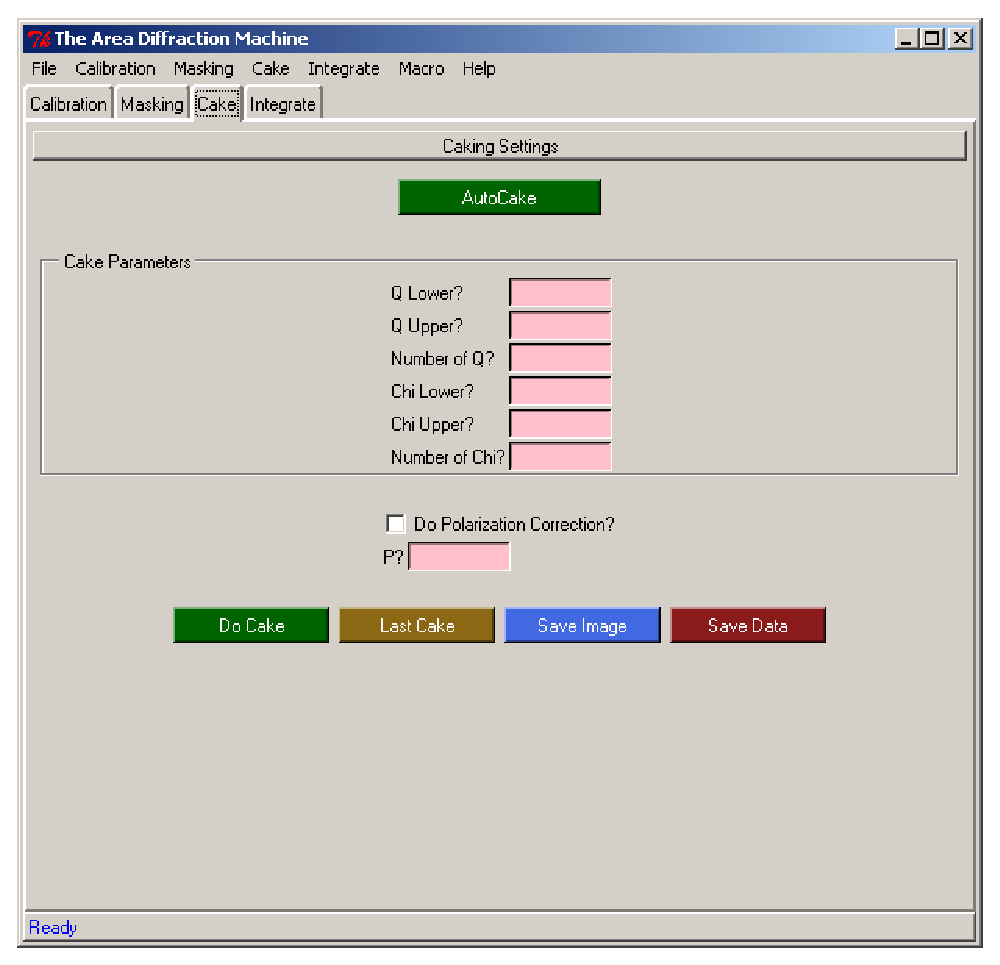
\includegraphics[scale=.75]{figures/caking_page.eps}
\caption{A screen shot of the caking tab to the program.
    This is the tab where you can cake data.} 
\label{caking_page}
\end{SCfigure}


In order to perform a cake with the program, you will have
to already have load into the program one or more
diffraction data files and you will have to input
calibration data into the program. Figure~\ref{caking_page}
shows the \gui{Caking} tab. This is where caking is done. 
In order to cake the data, the program will need to know a range
in $Q$ and $\chi$ space that should be caked. 
This can be inputted with the \gui{Q Lower?}, \gui{Q Upper?}
\gui{Chi Lower?}, and \gui{Chi Upper?} inputs.
It will also need to know how many $Q$ and $\chi$ bins to 
create when creating the caked data. This can be inputted
with the \gui{Number of Q } and \gui{Number of Chi} inputs.
Once this is done, you can push the 
\gui{Do Cake} button to cake the data. 

\begin{SCfigure}[1][htb]
\centering
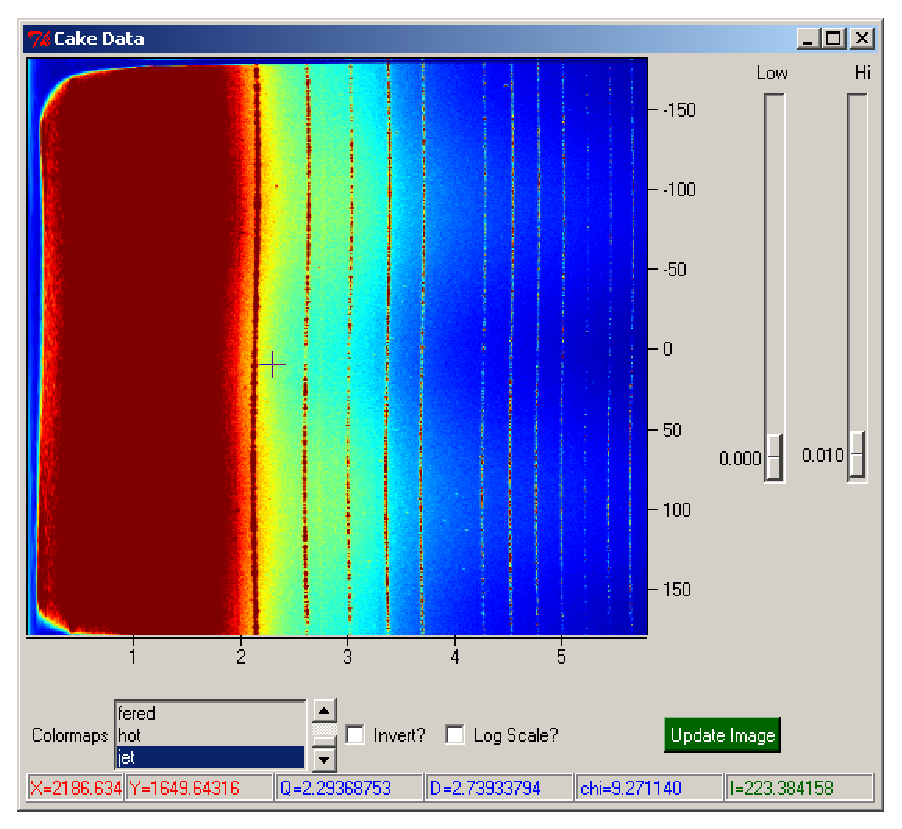
\includegraphics[scale=.75]{figures/cake_data_window.eps}
\caption{A screen shot of the cake data window for
    the program. This window will open up after the
    data is caked. This window behaves exactly like 
    the diffraction data window.} 
\label{cake_data_window}
\end{SCfigure}
After the caked data is created, the progarm will open up a cake data
window which displays the cake data interactively.
The cake data window is just like the diffraction
data window so everythign said in Chapter~\ref{viewing_data} 
carries over. The only real difference is that whenever
you zoom into the caked data, the program will take the user
selected zoom range and put it into the range inputs on
the cake page.

\section{AutoCake}

The program also has the convenience button \gui{AutoCake}.

To undo to whatever range was previously used when caking, 
\gui{AutoCake} will ``guess'' a good range of $Q$ and $\chi$ 
values, put them into the input, and then push the 
\gui{Do Cake} button for you. This lets you get out a 
cake without much work. What hte program thinks is a
good range is one that will put every pixel from the 
diffraction image into the cake. It will than pick
the bins sizes so that each pixel of the displayed 
cake data will correspond to its own bin. This will ensure
that the cake looks as sharp as the computer can draw it.
After the display is resized, the number of bins will
change correspondingly so that the next time you push
\gui{AutoCake} it will make the cake window look sharp again.

\section{Masking}

\section{Displaying Q lines and Peaks}
If a $Q$ list has been loaded into the program, 
$Q$ and $\Delta Q$ lines can be displayed on top
of the cake data. Remember that $Q$ lines on the
caked plot are just straight lines. 



\begin{figure}
    \centering
    \subfloat[A bad calibration]{
    \label{bad_calibration}
    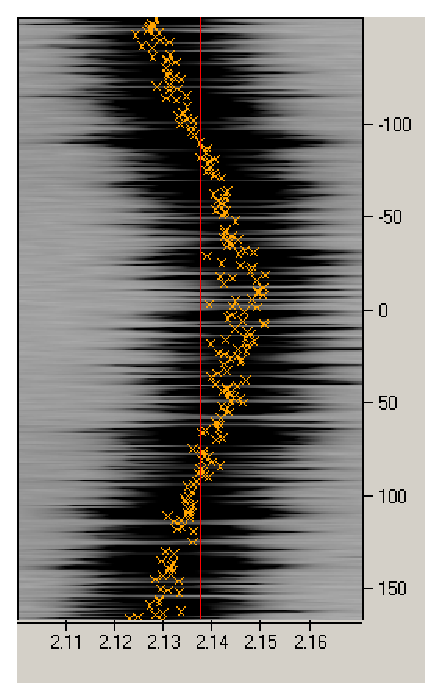
\includegraphics[scale=.75]{figures/bad_calibration.eps}}
    \subfloat[A good calibration]{
    \label{good_calibration}
    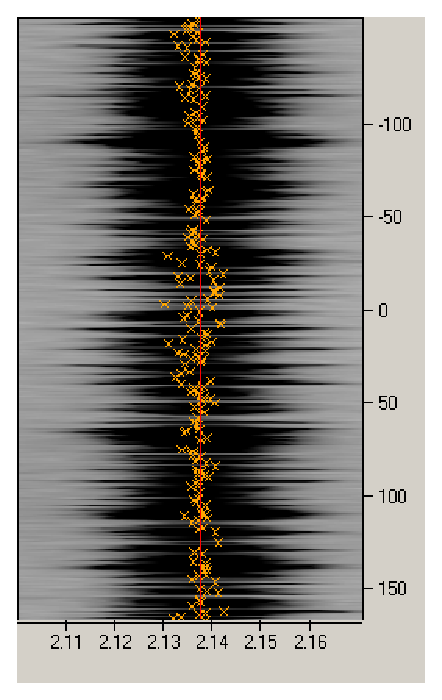
\includegraphics[scale=.75]{figures/good_calibration.eps}}
    \caption{A use of displaying peaks on top of the caked 
    data. Displaying the peaks found while calibrating can 
    be used to help tell if a proper calibration of caked 
    data has been done. Ideally, all the peaks will cluster 
    very close to the $Q$ line and there will be no systematic 
    variation of the peaks around the $Q$ value. If a bad 
    calibration was done, there will be this sort of
    distortion. This can easily be used to test if the
    program is properly calibrating your data.}
\label{calibration_cake}
\end{figure}

Also, any peaks that the program finds when performing
a calibration can be displayed on top of the caked
data. This can actually be very useful for checking if
a calibration was done properly.
figure~\ref{calibration_cake}. 

\section{Polarization Correction}
The program can apply a polarization correction to the
cake. To apply a polarization correction, you have
to check the \gui{Do Polarization Correction?} checkbox
and then input the value into the \gui{P?} input.

PUT MORE DISCUSSION HERE

\section{\texorpdfstring{Working in $2\theta$}{Working in 2theta}}

You can do everything related to caking in the variable
$2\theta$ instead of $Q$. To do so, you can go into
the file menu and select \gui{Work in 2theta}. When you 
do this, all of the names in the program will switch 
from $Q$ to $2\theta$. You will be asked to input 
$2\theta$ Lower, $2\theta$ Upper, Number of $2\theta$. 
The program will then display the cake image with
$2\theta$ as its axis.

\section{Saving Cake Images}

you can use the \gui{Last Cake} button to go back to the
previous cake values. You can also get at these values by 
right clicking on the caked window. (This is just like
zooming out of the diffraction window). You can save caked
data out as a jpg, gif, eps, pdf, bmp, png, or tiff.
When you save out the image as a popular image format, it
will save out the cake image with whatever threshold masks,
polygon masks, $Q$ lines, $\Delta Q$ lines, and peaks that
were displayed over the caked data as it is displayed by
the program.

\section{Saving Cake Data}

You can also save out the caked data in plain text. To do so,
you just have to push the \gui{Save Data} button and
select where to save it. The format of the file is a really
long comment string followed by the data 

\begin{lstlisting}[caption={'The Cake Data Header'}]
# Cake of: N:/data/LaB6_14_02_56.mar3450 
# Data Caked on Wed Mar 12 21:30:55 2008
# Calibration data used to make the cake:
#   x center:    1725.0000000 pixels
#   y center:    1725.0000000 pixels
#   distance:     125.2960000 mm
#   energy:     12735.3957721 eV
#   alpha:          0.0000000 degrees
#   beta:           0.0000000 degrees
#   rotation:       0.0000000 degrees
#   pixel length:     100.0000000 microns
#   pixel height:     100.0000000 microns
# A Polarization correction was applied
#   P = 0.500000
# A greater than mask was applied
#   Greater than mask = 1000.000000
# A Less Than Mask was applied
#   Less than mask = 10.000000
# Polygon mask(s) were applied
# Polygon(s) used in the analysis:
#   2400.10912343	1073.5706619
#   962.511627907	2282.88014311
#   2850.51520572	2572.86762075
#
#   1573.33631485	1215.47942755
#   1820.13416816	2893.70483005
#   2906.04472272	1573.33631485
# Cake range:
#   Q Lower = 0.000000
#   Q Upper = 6.726544
#   Number of Q = 560.000000
#   Q Step = 0.012012
#   chi Lower = -180.000000
#   chi Upper = 180.000000
#   Number of Chi = 560.000000
#   chi Step = 0.642857
# Note: pixels outside the diffraction image are saved as -1
#   Pixels greater than the greater than mask are saved as -2
#   Pixels less than the less than mask are saved as -3
#   Pixels inside of a polygon masks are saved as -4
# chi increased down. Q increases to the right
\end{lstlisting}
As you can see, the comment string is supposed to be as verbose
and useful as possible. The idea was to put into it as much
information about possible about under exactly what conditions
the cake was done. The first thing in the comment string is
the name of the file that was caked. If multiple files were loaded
and the sum image was caked, all of the files will be put into
the comment string. Next is a printout of the calibration values
used while caking the data. Next is the polarization correction,
greater than mask and less than mask that were used. It will print
out the pixel coordinates of any polygons that were applied to
the cake image. It prints out the cake range that is used.

Finally, the program codes special bins in the output caked data
with special values. Any bins that are outside of the diffraction
image in cake space are saved as -1. Any bins that were masked
because they were too large are saved as -2. Any bins that
were masked because they were too small are saved as -3. Any bins 
that were inside of a pixel maks are saved as -4. This is all
displayed in the comment string. The program tries to be smart about
the comment string. If no polygon masks were used, the comment string
instead contains lines like
\begin{lstlisting}[caption={'Alternate Header'}]
# No polarization correction was applied
# No greater than mask was applied
# No less than mask was applied
# No polygon masks were applied
\end{lstlisting}
If the program is working in $2\theta$ mode, the inputs will instead 
say \gui{2theta Lower}, etc. The comment string will instead have
\begin{lstlisting}[caption={'Another Alternate Header'}]
#   2theta Lower = 0.000000
#   2theta Upper = 62.814525
#   number of 2theta = 560.000000
#   2theta Step = 0.112169
\end{lstlisting}
Following the comment string is the data. The format for the data is
that each line corresponds to a different $\chi$ bin and each of the 
values for a particular $Q$ bins is separated by a space. Just
as the comment string explains, chi increased down and Q increases to 
the right. 





\chapter{Intensity Integration}
\index{Intensity Integration}
\section{The Integration Algorithm}

The purpose of performing an intensity integration is 
to create a plot of average intensity as a function
of either $Q$, $2\theta$, or $\chi$. The algorithm
for performing an intensity integration is pretty
straight foreward. In order to perform an intensity
integration, we must already know the calibration values
of the experiment for the paritcular image that will
be integrated. Than, a range and bin size for the
integration must be give. For example, you might
want to do a $Q-I$ integration from 2 to 5 with
100 bins. Whatever the range is, it 
must be specified before an integration is done.

The algorithm for performing the intensity integration
is as follows: loop over every pixel in the image. 
Add its intensity to the bin if it should be
in the bin based upon its value of $Q$, $2\theta$, or 
$\chi$. Remember that we need to use the calibration
values to calculate the correspondign $Q$, $2\theta$, and 
$\chi$ value using equation~\ref{ytermsydoubleprime}
\ref{xtermsxdoubleprime}, \ref{chitermsyx}, 
\ref{2thetatermsr}, and \ref{qterms2theta}.
After going through all the pixel, the bins then get averaged 
together. 

This program can constran the integration. 
This means that you can perform, for example,
a $Q$ integration of only those pixels with some
particular range of $\chi$ values. Or, you can
constaint your $\chi$ integration to on a particular
$Q$ range. This could be used, for example, to
perform a $\chi$ integration of only a particular
diffraction peak. The algorithm for performing
the constaint isn't any more complicated. You just
only bin a particular intensity value if it is
allowed by the constraint.

The program can allows for masking of pixels.
This complicates the algorithm a little bit further.
Whenever the program finds an intensity value
that should be masked (either because it is too 
large, too small, or in a polygon mask), it makes
sure not to bin that pixel and acts as though
it does not exist..

Finally, the program can perform a polarization 
correction to the integration. The polarization 
correction formula is
\begin{align}
    I&=Im/PF \\ 
    PF&=P(1 - (\sin(2\theta)\sin(\chi-90))^2) + 
    (1 - P)(1 - (\sin(2\theta)\cos(\chi-90))^2)
\end{align}
with $Im$ the measured intensity. If this
is selected, what happens
then is that all pixels have their intensity
value corrected by this formula before they
are binned. Note that the $2\theta$ and $\chi$
values correspond to the particular value
that is being corrected.

\section{Integrating with the Program}

All of the intensity integration is 


\chapter{Pixel Masking}
\index{Pixel Masking}

When analyzing diffraction data using this program,
not all of the pixels in an image have to be used in
the data analysis. In order to make the program
ignore certain pixels when doing the analysis, this
program allows for two types of pixel masking:
threshold masking and polygon masking. You can apply
a mask to a diffraction image by going to the
\gui{Masking} tab of the GUI. There is a screen
shot in figure~\ref{masking_page} of this tab.


\subsection{Threshold Masking}

\begin{SCfigure}[1][htb]
\centering
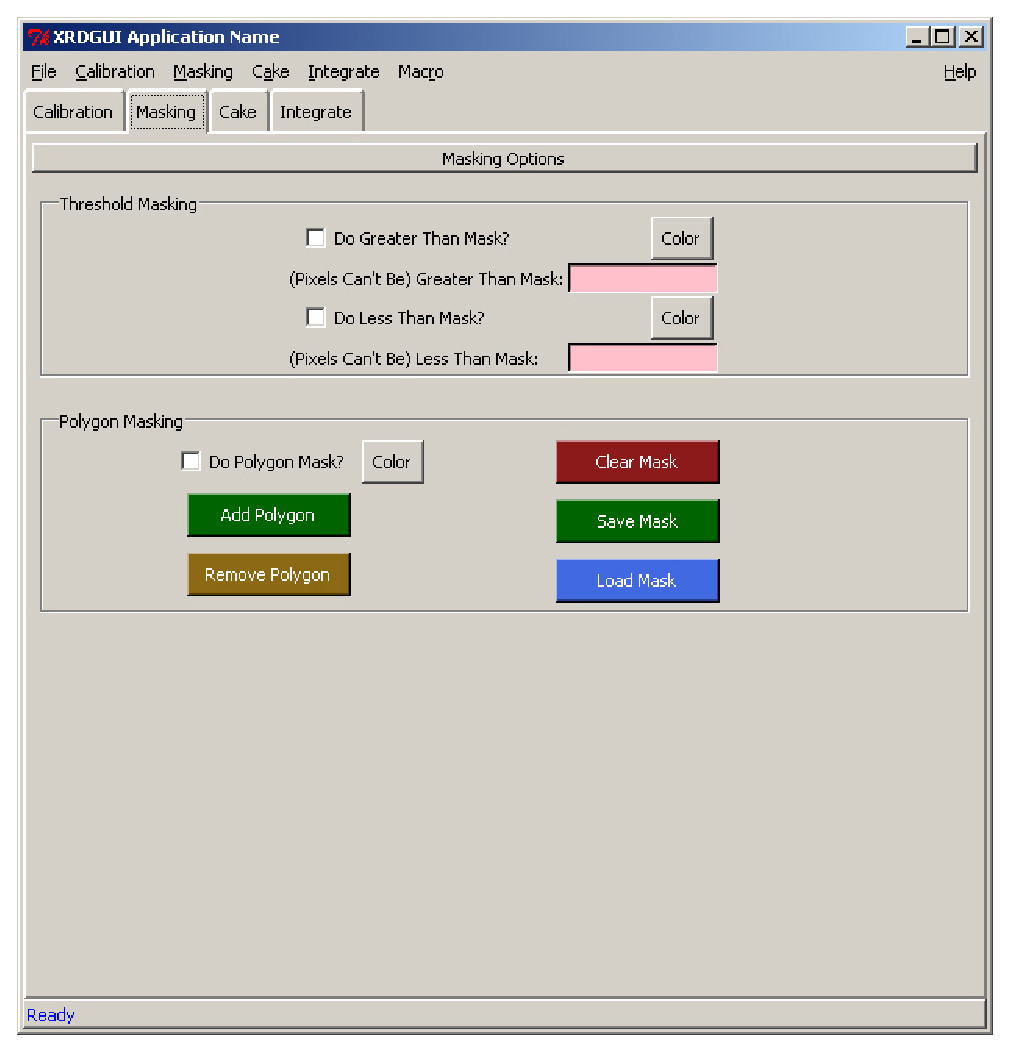
\includegraphics[scale=.75]{figures/masking_page.eps}
\caption{The page of the GUI for pixel masking. This 
page allows for threshold masking and polygon masking. 
Threshold masking can be used to have the program 
ignore all pixels with intensity above or below
a certain value when doing data analysis. 
Polygon masking can be used to have the programme
ignore all pixels in certain areas of the image
when doing data analysis.} 
\label{masking_page}
\end{SCfigure}

The top half of the \gui{Masking} tab is devoted to 
threshold masking. Threshold masking allows all pixels, 
either above a certain intensity value or below a certain 
intensity value, to be ignored when doing diffraction 
analysis. If you want to apply a mask that will cause 
all pixels greater than a certain value to be ignored,
you can select the \gui{Do Greater Than Mask?} option.
The \gui{(Pixel's Can't Be) Greater Than Mask} input 
lets you specify what the maximum pixel should be.
Correspondingly, the \gui{Do Less Than Mask} check box
allows you to require that the program ignores all
pixels below a certain value when doing diffraction
analysis. The lowest value can be specified by the 
\gui{Less Than Mask} input. 

\begin{SCfigure}[1][htb]
\centering
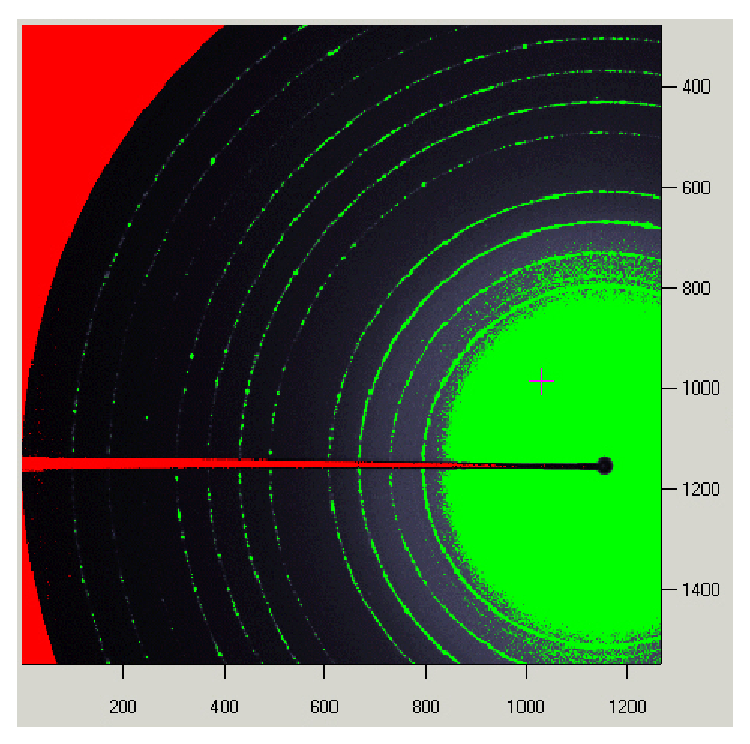
\includegraphics[scale=.75]{figures/Threshold_Masking.eps}
\caption{Here is an example of diffraction with a
greater than mask and less than mask applied.
All pixels in this image with intensity greater than 5000 
have been colored green. All pixels in this image with 
intensity less than 30 have been colored red. Applying
an intensity mask can be a useful way to see if a detector's
pixels have been overloaded and it can also be used to
ensure that no overloaded pixels are used in subsequent
data analysis.}
\label{Threshold_Masking}
\end{SCfigure}


When you apply a threshold mask, the pixels over this threshold 
will be colored differently on the diffraction and cake image. 
You can specify what color you want these masked pixels to show 
up as by with the \gui{Color} selector button next to the greater 
than and less then masks. Figure~\ref{Threshold_Masking} shows 
what the diffraction image looks like when all the pixels with 
intensity above 5000 were masked 
and colored green and all pixels below 30 were masked and
colored red.

If you apply a greater than mask and then save the cake data
to a file, any of the pixels that are larger than the greater
than mask are outputted with value -2. If you apply a less 
than mask and then save the cake data, any of the pixels
that are smaller than the less than mask are saved as -3.
If you need to analyze caked data further on, you need to
make sure to account for this. When you apply a threshold
mask and then perform an intensity integration, any of the 
too high or too low pixels are simply ignored when calculating
average intensity. 

\subsection{Polygon Masking}


\begin{SCfigure}[1][htb]
\centering
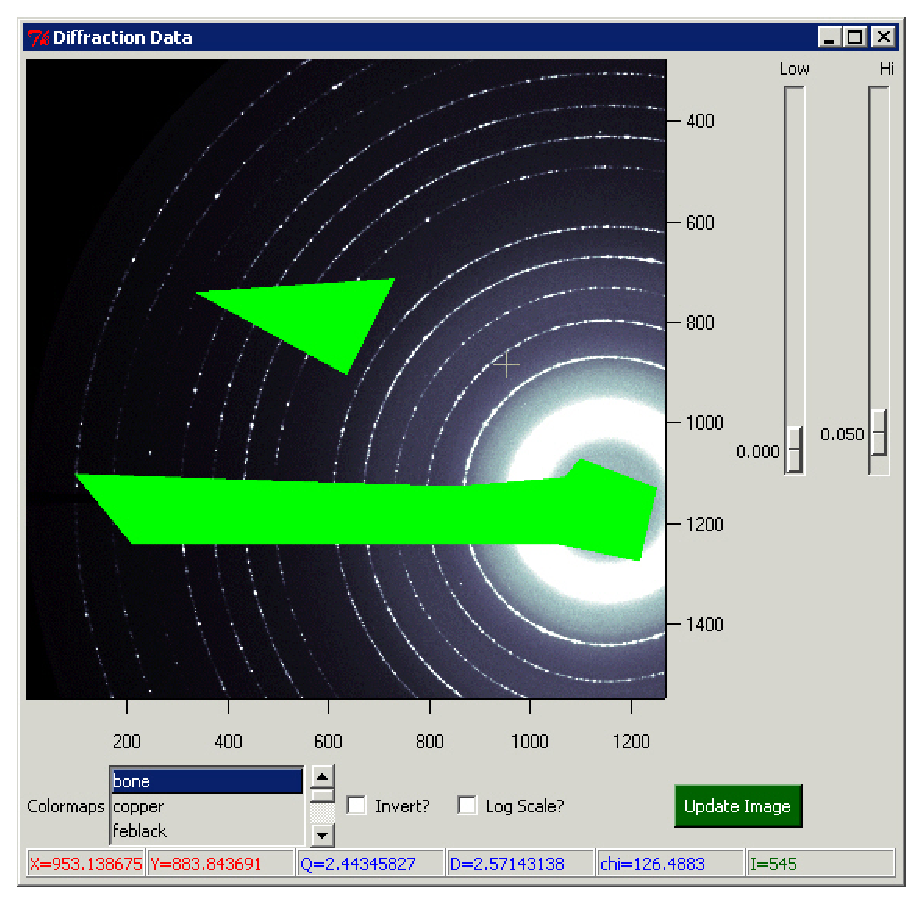
\includegraphics[scale=.75]{figures/Displayed_Polygon.eps}
\caption{In this screen shot of a diffraction image, we
see two polygon masks that have been added to the
image. One of them is blocking the beam stop and
the other is just there for show. Note that this program 
can use multiple polygons.}
\label{Displayed_Polygon}
\end{SCfigure}


Sometimes, large areas of a diffraction image are bad 
and should not be used in any data analysis. For example, 
often a beam stop blocks part of the diffraction data 
and the pixels which were blocked by the beam stop 
should be ignored. Also, sometimes parts of the experimental 
setup can block parts of the detector and those areas 
of the data must be ignored. This is called shadowing.
To allow for this sort of masking, the program has a 
polygon masking feature. You can draw polygons around 
certain parts of the diffraction image and those parts 
of the image will not be used in any diffraction analysis. 
The program can handle as many separate polygons as you 
want to use.

Once polygons have been added to the image (as is 
described below), you can have these polygons
used when performing data analysis by checking the
\gui{Do Polygon Mask?} check box. Once you do that,
these polygons will be displayed on the diffraction
and cake image. This is to say that any pixel in
the diffraction or cake image that is inside of one of
the polygons will be displayed with a different color.
An example of polygons on a diffraction image are 
shown in figure~\ref{Displayed_Polygon}.

You can change this color using the \gui{Color} button
next to the \gui{Do Polygon Mask?} check box.
When you save out cake data, any pixels inside of 
a polygon mask will be given an intensity 
value of -4. When you perform an intensity integration,
any of the masked pixels will simply be ignored when
calculating average intensities.

\begin{SCfigure}[1][htb]
\centering
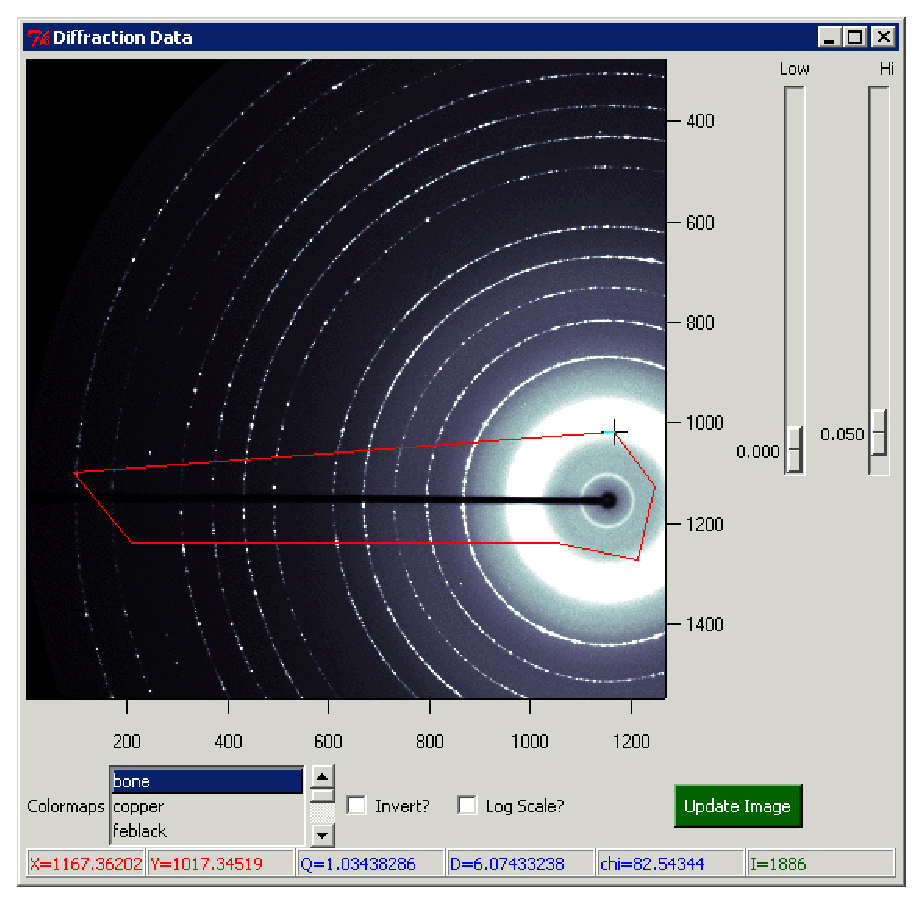
\includegraphics[scale=.75]{figures/Adding_Polygon.eps}
\caption{Here is a screen shot of the diffraction
image where the user is adding a new polygon 
mask that will be added into the program.
This mask will completely cover up the beam stop
and ensure that those values are not later used
when performing an intensity integration.}
\label{Adding_Polygon}
\end{SCfigure}

To add a polygon mask to the image, you have to push
the \gui{Add Polygon} button. When you push it, this
button will stay stuck. So pushing it enters you into
polygon drawing mode. When you are in this mode, 
the diffraction image will behave differently. You will not
be able to do any zooming or panning on the image. Instead,
when you left click on the diffraction image, you will 
begin drawing the polygon. The first left click on the
image will add the 
first vertex of the polygon. Each success left click
will add another vertex to the polygon. When you want to
finish drawing the polygon (by adding one final vertex to
it), you right click where you want that final polygon to
be. Once you right click, the program will exit the 
\gui{Add Polygon} mode and the regular zooming features of
the diffraction image will take over.
That polygon will then be added to the program. 
You can add as many polygons to the 
program as you wish. An example of drawing a 
polygon is shown in figure~\ref{Adding_Polygon}.
If you are are part way through drawing a polygon 
and decide that you don't like it any more, you can
simply unpush the \gui{Add Polygon} button and the
polygon in progress will be removed and the regular
bindings will take over.


\begin{SCfigure}[1][htb]
\centering
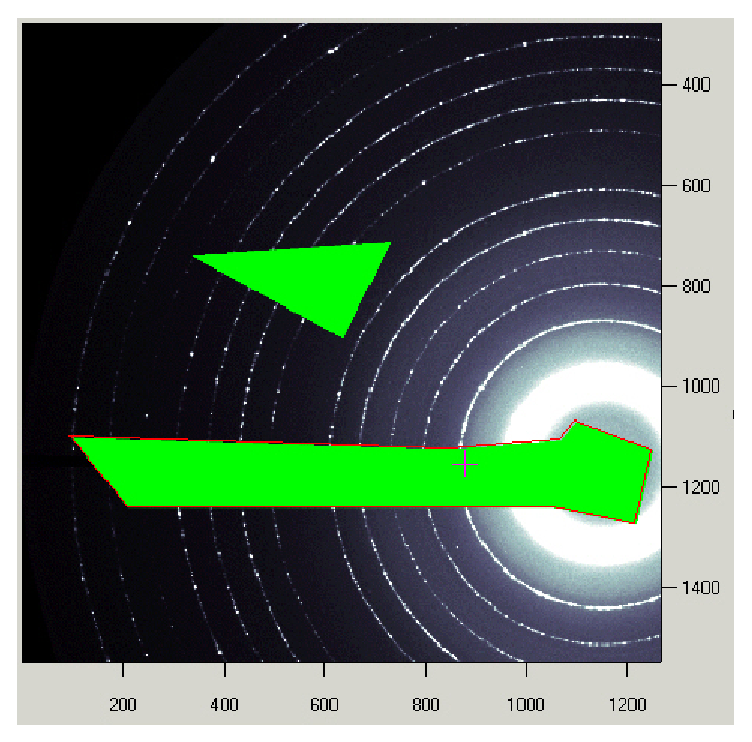
\includegraphics[scale=.75]{figures/Removing_Polygon.eps}
\caption{Here is a screen shot of the diffraction
image where the user is in the process of removing
a polygon. To remove a polygon, you have to push the
\gui{Remove Polygon} button and then click on the
polygon in the diffraction image that you want to
remove. When you mouse over a polygon,
the program will display a border around it so that
you know that that particular polygon is the one
that will be deleted.}
\label{Removing_Polygon}
\end{SCfigure}


If you want to remove a polygon that is already in
the program, you can push the \gui{Remove Polygon}
button. Like the \gui{Add Polygon} button, this
button will stay pushed and change the bindings of 
the diffraction image. When you now click on the
diffraction image while the mouse is on top of a
polygon, that polygon will be removed from the file.
After deleting a polygon, the program will leave
the \gui{Remove Polygon} mode and diffraction 
image will regain the regular zoom features.
An example of removing a polygon is shown
in figure~\ref{Removing_Polygon}
If you have a change of heart after pushing the
\gui{Remove Polygon} button and no longer want to
remove a polygon, you can simply unpush the button
and the program will leave the \gui{Remove Polygon}
mode. A gotcha that can easily happen when you are
using the diffraction image is that you push the
\gui{Add Polygon} or \gui{Remove Polygon} button
and then forget that you pushed it. If you do so,
the diffraction image will start behaving as
previously described. Don't forget that you can 
always unpush the button to return the program to
its normal state.

If you want to remove all the polygons in one go,
you can use the \gui{Clear Mask} button. If you
want to save all the polygons inside of the 
program to a file, you can use the \gui{Save Mask}
button. If you want to load all of the polygons
from a file into the program, you can use the
\gui{Load Mask} button. The file format for polygon
mask files is very simple. For example, saving
out the polygons shown in figure~\ref{Displayed_Polygon}
creates the file:
\begin{lstlisting}[caption={'A demonstrative polygon mask file'}]
# Polygon(s) drawn on Thu Feb 07 00:00:21 2008
93.140587183	1098.06704199
208.013978042	1237.77792276
1052.48863517	1237.77792276
1213.93231962	1271.92947139
1248.08386825	1126.00921814
1095.95424252	1067.02017959
1064.90738013	1104.27641447
847.579343365	1122.9045319

332.201427619	737.923438212
633.355992844	902.471808902
729.601266267	709.981262058
\end{lstlisting}
The format for these files is to have each line have
an ($x$,$y$) coordinate for one of the nodes in
the polygon. Multiple polygons are separated by
newlines and there should be no other formatting.
Note that as in figure~\ref{Displayed_Polygon},
one of the polygons has only three vertices
and is a triangle while the other has many
vertices and is a more complicated shape.
As always, comment lines beginning with \# are 
ignored except when they are between coordinates
in which case they also signify the division of
separate polygons.




\chapter{Macros}
\index{Macros}
\chapter{Macros}

This program is almost fully automatable with macros. Macros
can be used to quickly analyze data. 
This program is capable of recording and running macros and
it is easy to write and modify macro files. 

\begin{SCfigure}[1][hbtp]
    \centering
    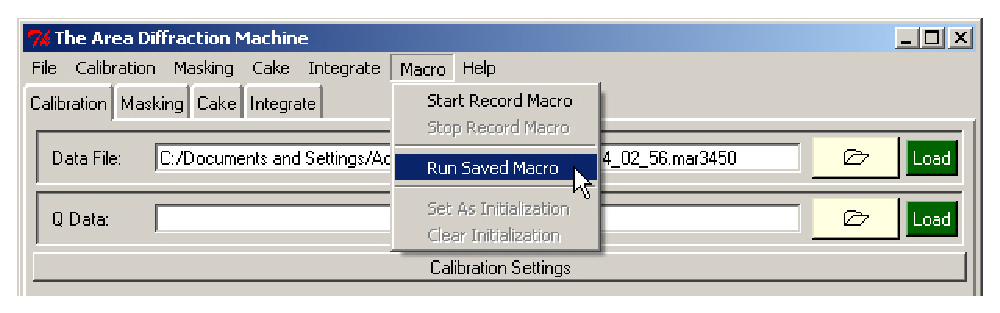
\includegraphics[scale=.75]{figures/macro.eps}
    \caption{The \gui{Macro} menu bar is used to
    record and run macros.}
    \label{macro_figure}
\end{SCfigure}

\section{Record and Run Macros}

The easiest way to create a macro is to record it by selecting 
the \gui{Start Record Macro} 
option in the \gui{Macro} menu 
bar shown in  figure~\ref{macro_figure}. 
After all of the desired steps are finished, 
the \gui{Stop Record Macro} option will save the macro to
a file. The \gui{Run Saved Macro} option in the \gui{Macro}
menu will run all the commands in a saved macro. 

\section{The \gui{Abort} Button}

Version 2 of the program introduces an abort button which
can be used to abort out of running a macro in the middle
of running it. Figure~\ref{macro_figure} shows a screen shot
of this button. This can be useful if part way through
running a long macro, you realize that the macro isn't
doing the right thing. It is sometimes a little difficult to 
push the button and have it actually stop the program, especially 
when the program gets frozen up running long calculations like an 
intensity integration, but if you are diligent and push it a couple 
of times, it will eventually stop the macro. 

\begin{SCfigure}[1][hbtp]
    \centering
    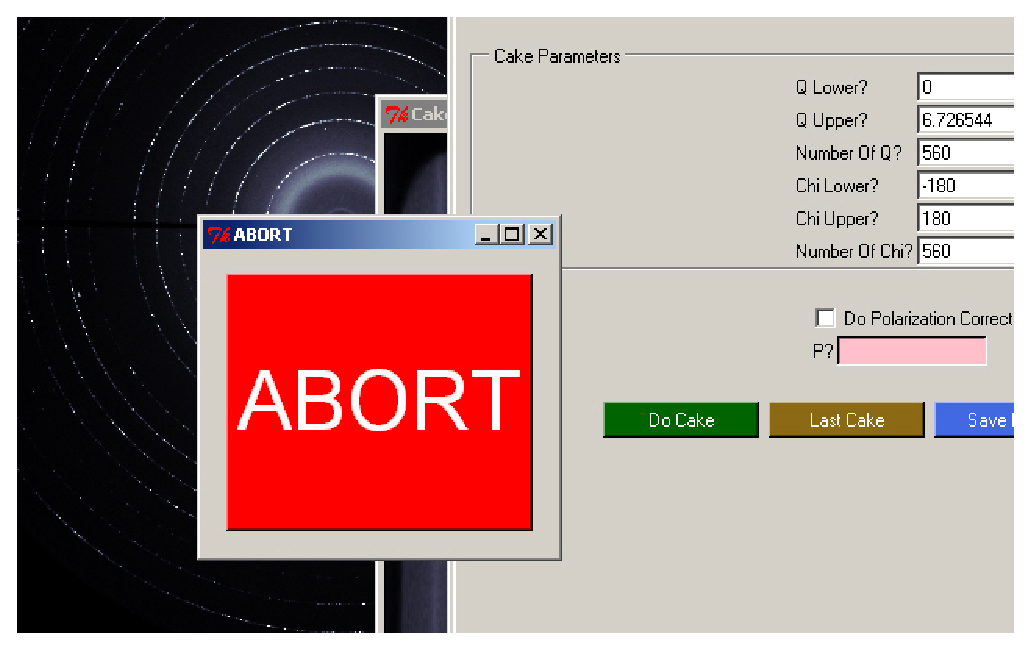
\includegraphics[scale=.75]{figures/abort_button.eps}
    \caption{The \gui{Abort} button can be used to abort
    out of a running macro.}
    \label{abort_button}
\end{SCfigure}

\section{\texorpdfstring{The \gui{Set As Initialization} Option}
    {The ``Set As Initialization'' Option}}
    \label{setAsInitializationSection}

Version 2 of the Area Diffraction Machine introduces the
feature \gui{Set As Initialization}. It can be used to run
a particular Macro file ever time the Area Diffraction Machine
is opened. This is a useful way to make the program always open
with certain options selected and certain inputs set to particular
values (like setting the \gui{Stddev?} input to 7).
The best way to do this is to open the program, start recording a macro
set the program in the desired state, and instead of pushing
the \gui{Stop Record Macro} button push the 
\gui{Set As Initialization} option. This will save the recorded macro to
the file \gui{InitializationMacro.dat} in the folder
\gui{Preferences/} next to the executable.\footnote{It
is a little bit harder to find this file on the Macintosh.
To find it, right click on the application and 
select the \gui{Show Package Contents}
option. Inside of the \gui{Contents/} folder is the folder 
\gui{Resources/} which contains the \gui{Preferences/} folder where
you can find the file}. If desired, the \gui{InitializationMacro.dat}
file can be modified by hand to change the macro file. 

To get the program to no longer run a macro whenever the program opens,
either push the \gui{Clear Initialization} option next to the
\gui{Set As Initialization} option. Alternately, push the
\gui{Start Record Macro} option and then immediately push the 
\gui{Set As Initialization} option. Alternately, simply
delete the \gui{InitializationMacro.dat} file.


\section{The Macro File Format}

A macro file is a list of commands, each on their own line, that tells the 
program what to do.
The syntax for macros is straightforward. Macro commands are the 
text corresponding to the part of the GUI that does 
the command. 
For example, the macro command \macroline{Get From Header} 
will get the calibration data from the header of the 
image.\footnote{Because of the ambiguity of some GUI items,
some macro command have different names. 
For example, the \gui{Number Of Chi} input shows up multiple
places in the program so the macro commands are instead
\macroline{Fit Number of Chi?}, \macroline{Integrate Number Of Chi?},
and \macroline{Cake Number Of Chi?}. When in doubt, 
section~\ref{macro_commands_table} has a list of all macro commands.}
Things get more interesting when the GUI item is more complicated
then a button. The \gui{Draw Q Data?} check box needs to know if it 
is selected or deselect. The macro command is
\begin{lstlisting}
Draw Q Data?
    Select
# Or, Deslect to not display them
\end{lstlisting}
Entering numbers is similar:
\begin{lstlisting}
beta:
    5.23
\end{lstlisting}
So are filenames:
\begin{lstlisting}
Save Caked Image
    C:/cake_output.jpg
\end{lstlisting}

\section{Looping Over Diffraction Data}
\label{LoopOverDiffractionData}

Diffraction data is loaded with the command
\begin{lstlisting}
Data File:
    C:/foo.mar3450
\end{lstlisting}
Diffraction files in a list will be looped over and the same
analysis can be performed on all of them.
For example,
\begin{lstlisting}
Data File:
    C:/foo.mar3450 C:/bar.mar3450 
# ...
\end{lstlisting}
will run the subsequent macro lines on
the file \macroline{C:/foo.mar3450} and
then on the file \macroline{C:/bar.mar3450}.
The loop will end when one of three things happens: a subsequent line 
in the macro file is \macroline{END LOOP}, more diffraction data
is loaded using the \macroline{Data File:} command, or
the macro file ends. 

Directories can also be given. The program 
will (non-recursively) look for all diffraction
files in the directory and include them in the list. If the folder
\macroline{C:/data} contained the file \macroline{foo.mar3450}
and \macroline{bar.mar3450}, these files could
be looped over with the command
\begin{lstlisting}
Data File:
    C:/data/
# ...
\end{lstlisting}
Multiple folders and multiple files can be in the list.
They must be on the same line and separated by spaces.

\section{PATHNAME and FILENAME}

When a diffraction file is loaded by the macro,
any subsequent lines in the file will have
the string \macroline{PATHNAME} replaced with the
path of the current diffraction file and 
\macroline{FILENAME} replaced with the filename
of the current diffraction file.
For the file \macroline{C:/data/first.mar3450},
\macroline{PATHNAME} would be replaced by
\macroline{C:/data} and \macroline{PATHNAME} would
be replaced by \macroline{first}. A \macroline{.mar3450}
file could be reconstructed as 
\macroline{FILENAME/PATHNAME.mar3450}

While looping over multiple files, these commands can be used to
save things in useful places with useful names. It would be
easy, for example, to save intensity integrated data with the
macro:
\begin{lstlisting}
Save Integration Data
    FILENAME/PATHNAME\_int.dat
\end{lstlisting}
This would save the intensity data for
\macroline{C:/data/foo.mar3450} as
\macroline{C:/data/foo\_int.dat} and
the intensity data for \macroline{C:/data/bar.mar3450} as
\macroline{C:/data/bar\_int.dat}, etc. 

\section{Loading Multiple Images}

Multiple diffraction files can be loaded and their 
intensities added. The macro command to do this is
\macroline{Multiple Data Files} followed by a list of filenames
enclosed with [ and ] brackets. 
\macroline{C:/data/foo.mar3450} and
\macroline{C:/data/bar.mar3450} could be loaded at the
same time with the macro
\begin{lstlisting}
Multiple Data Files:
    [C:/data/foo.mar3450 C:/data/bar.mar3450]
# ...
\end{lstlisting}
All of the files that are added together must be in the same folder
so that that the \macroline{PATHNAME} syntax remains 
meaningful.
These sets of files can be looped over by putting
several of these bracketed lists on a line.
For example:
\begin{lstlisting}
Multiple Data Files:
    [C:/a.mar3450 C:/b.mar3450] [C:/c.mar3450 C:/d.mar3450]
# ...
\end{lstlisting}
will separately loop over \macroline{a.mar3450} 
and \macroline{b.mar3450} added together and then 
\macroline{c.mar3450} and \macroline{d.mar3450}
added together. Alternately,
all of the files that need to be analyzed can be grouped into 
subfolders. If each subfolder contains only files that should
be added together, the \macroline{Multiple Data Files} command
followed by the base folder will loop over each of the subfolders
and add all of the files in each subfolder together.
For example, the folder \macroline{C:/data}
contained the sub folder \macroline{A} containing the files 
\macroline{a.mar3450} and \macroline{b.mar3450}
and suppose \macroline{C:/data} also contained the 
sub folder \macroline{B} containing the files
\macroline{c.mar3450} and \macroline{d.mar3450}.
The macro command
\begin{lstlisting}
Multiple Data Files:
    C:/data
# ...
\end{lstlisting}
would first load \macroline{a.mar3450} and 
\macroline{b.mar3450} and run the through loop.
It would then load \macroline{c.mar3450} and 
\macroline{d.mar3450} and run the through loop.
Multiple Lists of files and multiple
folders containing subfolders can be put after
the \macroline{Multiple Data Files} line. They
must all be on the same line and separated by spaces.
Since the all the files added together must come
from the same folder, \macroline{PATHNAME} is
unambiguous. \macroline{FILENAME} is replaced by the 
string \macroline{MULTIPLE\_FILES} to avoid ambiguity.

\section{FOLDERPATH and FOLDERNAME}

To facilitate writing macros that load and 
add together diffraction files in a loop, 
macros allow the \macroline{FOLDERNAME}
and \macroline{FOLDERPATH} syntax.
\macroline{FOLDERNAME} will be replaced
by the name of the folder containing the current
diffraction file(s). \macroline{FOLDERPATH} 
will be replaced by the path leading to the folder 
containing the file. A \macroline{mar3450}
file can be reconstructed as 
\macroline{FOLDERPATH/FOLDERNAME/FILENAME.mar3450}.
\macroline{FOLDERNAME} is useful because if multiple
files have been loaded at the same time, output can be saved
with the enclosing folder's name. If multiple subfolders
are looped over, the output of the program for each set of 
files can be given a meaningful name using the subfolder's
name.

\section{Setting Colors in a Macro}

There are several places in the program where a
color can be selected. Colors can be set from
inside a macro but the names of the colors is
a little confusing. The easiest way to figure out 
the macro command to set a color is to record a macro
and then copy and paste.
Technically, the program will accept 
any color string that the tk GUI framework accepts. tk
will accept quite a few colors by their English name (such as 
\macroline{red}).\footnote{\url{http://wiki.tcl.tk/16166} 
contains a list of all the allowed color names.} 
Tk also accepts colors
by their RGB value. A color is written as \#
followed by the color's RGB value in hexadecimal.
Each red, green, and blue value ranges from 0 to 255 in
decimal and 00 to ff in hexadecimal. For example, \#ff0000 is red. 

\section{Little Tidbits}\label{Little Tidbits}
\begin{itemize}
    \item Macro commands are not case
    sensitive. The command \macroline{GeT fRoM hEaDeR} 
    is just as valid as 
    \macroline{Get From Header}. 
    \item White spaces at the beginning and end of a
    line are ignored. In the preceding examples, the
    spaces separating macro commands from input values
    was only there to increase readability. 
    \item New lines in a macro file are ignored.
    \item Comment lines beginning with \# 
    are ignored.
    \item The program will automatically move
    between tabs as it executes different commands 
    on different tabs. 
    \item Usually, macro commands will not be recorded
    when the macro item is selected through the menu bar. The
    only exceptions are items that can only be accessed
    that way.
    \item The program will create folders if necessary in
    order to save files out into folders that are specified
    but that do not yet exist.
\end{itemize}


\section{List of Macro Commands}\label{macro_commands_table}

\begin{center}

\setlongtables % keeps the width uniform across pages
\begin{longtable}{|p{4cm}|p{4cm}|p{7cm}|}
\caption{Macro Commands} \label{grid_mlmmh} \\

\hline \multicolumn{1}{|c|}{Command} & \multicolumn{1}{c|}{Followed By} & \multicolumn{1}{c|}{Effect} \\ \hline 
\endfirsthead

\multicolumn{3}{c}%
{{\bfseries \tablename\ \thetable{} -- continued from previous page}} \\

\hline \multicolumn{1}{|c|}{Command} & \multicolumn{1}{c|}{Followed By} & \multicolumn{1}{c|}{Effect} \\ \hline 
\endhead

\hline \multicolumn{3}{|r|}{{Continued on next page$\ldots$}} \\ \hline
\endfoot

\hline 
\endlastfoot
\multicolumn{3}{|c|}{Program State Commands}\\
\hline 
    \macrolinenoquotes{Work In eV}&None&Changes the state of 
        the program to work with the beam's energy.\\
    \macrolinenoquotes{Work in Lambda}&None&Changes the state of 
        the program so that the beam's wavelength.\\
    \macrolinenoquotes{Work in 2theta}&None&Changes the state of
        the program so that caking and intensity integration
        are done in $2\theta$ instead of $Q$.\\
    \macrolinenoquotes{Work in Q}&None&Changes the state of
        the program so that caking and intensity integration
        are done in $Q$ instead of $2\theta$.\\
    \hline
    \multicolumn{3}{|c|}{Calibration Commands} \\
    \hline
    \macrolinenoquotes{Data File:}&Files \& Directories&Opens
        a diffraction file and possibly loops over doing this.\\
    \macrolinenoquotes{Multiple Data Files"}&
        Files \& Directories&Loads several 
        several diffraction files and adding
        them together and possibly loops over doing this.\\
    %\macrolinenoquotes{Dark Current:}&Filename&Loads in the 
    %    Dark Current.\\
    \macrolinenoquotes{Q Data:}&Filename&Load in a $Q$ data file.\\
    \macrolinenoquotes{Standard Q}&$Q$ File&Loads in a
    standard $Q$ files. This command is followed by the name 
    in the standard $Q$ menu of one of the standards.\\
    \macrolinenoquotes{Get From Header:}&None&Gets the calibration 
        data from the image header.\\
    \macrolinenoquotes{Load From File:}&Filename&Loads a calibration 
        data file.\\
    \macrolinenoquotes{Previous Values}&None&Loads the previous
        calibration parameters.\\
    \macrolinenoquotes{Save To File}&Filename&Saves the calibration 
        data to a file.\\
    \macrolinenoquotes{xc:}&Number&Sets the $x$ center.\\
    \macrolinenoquotes{xc Fixed:} & \selectordeselect & Sets whether 
        or not to fix the $x$ center.\\
    \macrolinenoquotes{yc:}&Number&Set the $y$ center.\\
    \macrolinenoquotes{yc Fixed:}& \selectordeselect &Sets whether 
        or not to fix the $y$ center.\\
    \macrolinenoquotes{d:}&Number&Set the detector distance.\\
    \macrolinenoquotes{d Fixed:}& \selectordeselect &Sets whether 
        or not to fix the distance.\\
    \macrolinenoquotes{E:}&Number&Sets the energy. If the 
        program is in $\lambda$ mode, it will switch to $eV$ mode.\\
    \macrolinenoquotes{E Fixed:}& \selectordeselect &Sets whether 
        or not to fix the energy. If the program is in $\lambda$ mode,
        it will switch to $eV$ mode.\\
    \macrolinenoquotes{lambda:}&Number&Sets the wavelength. If
        the program is in $eV$ mode, it will switch to $\lambda$ mode.\\
    \macrolinenoquotes{lambda Fixed:}& \selectordeselect &Sets 
        whether or not to fix the wavelength. 
        If the program is in $eV$ mode, it will switch to $\lambda$ mode.\\
    \macrolinenoquotes{alpha:}&Number&Sets the $\alpha$ angle.\\
    \macrolinenoquotes{alpha Fixed:}& \selectordeselect &Sets whether 
        or not to fix the $\alpha$ angle.\\
    \macrolinenoquotes{beta:}&Number&Sets the $\beta$ angle.\\
    \macrolinenoquotes{beta Fixed:}& \selectordeselect &Sets whether 
        or not to fix the $\beta$ angle.\\
    \macrolinenoquotes{R:}&Number&Sets the rotation angle.\\
    \macrolinenoquotes{R Fixed:}& \selectordeselect &Sets whether 
        or not to fix the rotation angle.\\
    \macrolinenoquotes{pl}&Number&Sets the pixel length.\\
    \macrolinenoquotes{ph}&Number&Sets the pixel height.\\
    \macrolinenoquotes{Draw Q Lines?}&\selectordeselect&Sets whether 
        or not to draw constant $Q$ lines.\\
    \macrolinenoquotes{Draw Q Lines Color?}&color&Sets the color 
        of the constant $Q$ lines.\\
    \macrolinenoquotes{Draw dQ Lines?}&\selectordeselect&Sets wheter
        or not to draw constant $\Delta Q$ lines.\\
    \macrolinenoquotes{Draw dQ Lines Color?}&color&Sets the 
        color of the $\Delta Q$ lines.\\
    \macrolinenoquotes{Draw Peaks?}&\selectordeselect&
        Sets wheter or not to draw the fit peaks.\\
    \macrolinenoquotes{Draw Peaks Color?}&color&Sets the color of 
        the peaks.\\
    \macrolinenoquotes{Update}&None&Refreshes the diffraction image.\\
    \macrolinenoquotes{Save Calibration}&Filename&Saves the
        calibration parameters to a file.\\
    \macrolinenoquotes{Do Fit}&None&Fits the calibration parameters.\\
    \macrolinenoquotes{Save Last Fit}&Filename&Introduces in version 2 of
        the program. Will save information about the previous calibration
        to a file.\\
    \macrolinenoquotes{Make/Save Peak List}&Filename&Creates a peak 
        list and saves it to a file.\\
    \macrolinenoquotes{Use Old Peak List (if possible)?}&
        \selectordeselect&Sets whether or not to use previous peak lists
        when fitting.\\
    \macrolinenoquotes{Fit Number of Chi?}&Number&Sets the number of 
        $\chi$ slices around the diffraction image used
        when calibrating.\\
    \macrolinenoquotes{Stddev}&Number&The threshold for 
        allowing peaks.\\
    \hline    
    \multicolumn{3}{|c|}{Diffraction Display Commands} \\
    \hline
    \macrolinenoquotes{Diffraction Data Colormaps}&A colormap name&
        Sets the colormap used to display the diffraction data.\\
    \macrolinenoquotes{Diffraction Data Invert?}&\selectordeselect&
        Inverts the colormap used to display the diffraction data.\\
    \macrolinenoquotes{Diffraction Data Log Scale?}&\selectordeselect&
        Sets whether or not to use a log of the colormap.\\
    \macrolinenoquotes{Diffraction Data Low?}&Number from 0 to 1&Sets
        the percentage of maximum intensity that is mapped to the 
        lowest part of the colormap.\\
    \macrolinenoquotes{Diffraction Data Hi?}&Number from 0 to 1&Sets
        the percentage of maximum intensity that is mapped to the
        highest part of the colormap.\\
    \macrolinenoquotes{Save Diffraction Image}&Filename&Saves the 
        diffraction image to a file.\\
    \hline    
    \multicolumn{3}{|c|}{Masking Commands}\\
    \hline
    \macrolinenoquotes{Do Less Than Mask?}&\selectordeselect&
        Sets whether or not to apply a less than mask to the
        diffraction data.\\
    \macrolinenoquotes{(Pixels Can't Be) Less Than Mask:}&Number&
        Sets the less than mask.\\
    \macrolinenoquotes{Less Than Mask Color?}&color&Sets the
        color of the less than mask.\\
    \macrolinenoquotes{Do Greater Than Mask?}&\selectordeselect&
        Sets whether or not to apply a greater than mask to the
        diffraction data.\\
    \macrolinenoquotes{(Pixels Can't Be) Greater Than Mask:}&
        Number&Sets the greater than mask.\\
    \macrolinenoquotes{Greater Than Mask Color?}&color&Sets
        the color of the greater than mask.\\
    \macrolinenoquotes{Do Polygon Mask?}&\selectordeselect&
        Sets whether or not to use polygon masks.\\
    \macrolinenoquotes{Polygon Mask Color?}&color&Sets
        the color of the polygon masks.\\
    \macrolinenoquotes{Save Mask}&Filename&Saves all 
        polygon masks to a file.\\
    \macrolinenoquotes{Load Mask}&Filename&Loads all
        polygon masks from a file.\\
    \macrolinenoquotes{Clear Mask}&None&Removes ll
        polygon masks.\\
    \hline
    \multicolumn{3}{|c|}{Cake Commands}\\
    \hline
    \macrolinenoquotes{AutoCake}&None&Picks a 
        nice $Q$ and $\chi$ range and cakes.\\
    \macrolinenoquotes{Cake Q Lower?}&Number&Sets the lower $Q$ value 
        used when caking. If the program is in $2\theta$ mode, 
        it will switch to $Q$ mode.\\
    \macrolinenoquotes{Cake Q Upper?}&Number&Sets the upper $Q$ value 
        used when caking. If the program is in $2\theta$ mode, 
        it will switch to $Q$ mode.\\
    \macrolinenoquotes{Cake Number Of Q?}&Number&Sets the number of 
        $Q$ bins used when caking. If the program is 
        in $2\theta$ mode, it will switch to $Q$ mode.\\
    \macrolinenoquotes{Cake 2theta Lower?}&Number&Sets the lower 
        $2\theta$ value used when caking. If the program is in 
        $Q$ mode, it will switch to $2\theta$ mode.\\
    \macrolinenoquotes{Cake 2theta Upper?}&Number&Sets the upper
        $2\theta$ value used when caking. If the program is in 
        $Q$ mode, it will switch to $2\theta$ mode.\\
    \macrolinenoquotes{Cake Number Of 2theta?}&Number&Sets the
        number of $2\theta$ bins used when caking. If the program 
        is in $Q$ mode, it will switch to $2\theta$ mode.\\
    \macrolinenoquotes{Cake Chi Lower?}&Number&Sets the lower $\chi$ 
        value used when caking.\\
    \macrolinenoquotes{Cake Chi Upper?}&Number&Sets the upper $\chi$ 
        value used when caking.\\
    \macrolinenoquotes{Cake Number Of Chi?}&Number&Sets the number of 
        $\chi$ values used when caking.\\
    \macrolinenoquotes{Do Cake}&None&Performs the cake and displays 
        that caked data.\\
    \macrolinenoquotes{Last Cake}&None&Goes back to the previous 
        cake values.\\
    \macrolinenoquotes{Save Caked Image}&Filename&Saves the
        cake as a popular image format. The extension
        of the file tells the program what format
        to save the image as.\\
    \macrolinenoquotes{Save Caked Data}&Filename&Saves
        the cake to a file.\\
    \macrolinenoquotes{Cake Do Polarization Correction?}&
        \selectordeselect&Sets whether or not to apply
        a polarization correction when caking.\\
    \macrolinenoquotes{Cake P?}&Number from 0 to 1&Sets the 
        value of the polarization used when
        caking.\\
    \hline    
    \multicolumn{3}{|c|}{Cake Display Commands} \\
    \hline
    \macrolinenoquotes{Cake Data Colormaps:}&Colormap&
        Sets the colormap used to display the caked data.\\
    \macrolinenoquotes{Cake Data Invert?}&\selectordeselect&
        Sets whether or not to invert the colormap used to
        display the caked data.\\
    \macrolinenoquotes{Cake Data Log Scale?}&\selectordeselect&
        Sets whether or not to use a log scale of the colormap.\\
   \macrolinenoquotes{Cake Data Low?}&Number from 0 to 1&Sets
        the percentage of maximum intensity that is mapped to the 
        lowest part of the colormap.\\
    \macrolinenoquotes{Cake Data Hi?}&Number from 0 to 1&Sets
        the percentage of maximum intensity that is mapped to the
        highest part of the colormap.\\
    \hline    
    \multicolumn{3}{|c|}{Intensity Integration Commands}\\
    \hline
    \macrolinenoquotes{Integrate Q Lower?}&Number&Sets the lower
    $Q$ value used when integrating.
    If the program is in $2\theta$ mode, it will switch to $Q$ mode.\\
    \macrolinenoquotes{Integrate Q Upper?}&Number&Sets the upper
    $Q$ value used when integrating.
    If the program is in $2\theta$ mode, it will switch to $Q$ mode.\\
    \macrolinenoquotes{Integrate Number Of Q?}&Number&Sets the number of
    $Q$ bins used when integrating.
    If the program is in $2\theta$ mode, it will switch to $Q$ mode.\\
    \macrolinenoquotes{Integrate 2theta Lower?}&Number&Sets the lower
    $2\theta$ value used when integrating.
    If the program is in $Q$ mode, it will switch to $2\theta$ mode.\\
    \macrolinenoquotes{Integrate 2theta Upper?}&Number&Sets the upper
    $2\theta$ value used when integrating.
    If the program is in $Q$ mode, it will switch to $2\theta$ mode.\\
    \macrolinenoquotes{Integrate Number Of 2theta?}&Number&Sets the number of
    $2\theta$ bins used when integrating.
    If the program is in $Q$ mode, it will switch to $2\theta$ mode.\\
    \macrolinenoquotes{Integrate Chi Lower?}&Number&
    Sets the lower $\chi$ value used when integrating.\\
    \macrolinenoquotes{Integrate Chi Upper?}&Number&
    Sets the upper $\chi$ value used when integrating.\\
    \macrolinenoquotes{Integrate Number Of Chi?}&Number&
    Sets the number of $\chi$ bins used when integrating.\\
    \macrolinenoquotes{Integrate Q-I}&None&Performs a 
    $Q$ integration. If the program is in $2\theta$ mode, it 
    will switch to $Q$ mode.\\
    \macrolinenoquotes{AutoIntegrate Q-I}&None&Picks
    a good range of $Q$ values and does a $Q$ 
    integration. If the program is in $Q$ mode, 
    it will switch to $2\theta$ mode.\\
    \macrolinenoquotes{Integrate 2theta-I}&None&Performs
    a $2\theta$ integration. If the program is in $Q$ mode, 
    it will switch to $2\theta$ mode.\\
    \macrolinenoquotes{AutoIntegrate 2theta-I}&None&
    Picks a good range of $2\theta$ values and does
    a $2\theta$ integration. If the program is in $Q$ mode, 
    it will switch to $2\theta$ mode.\\
    \macrolinenoquotes{Integrate chi-I}&None&Performs
    a $\chi$ integration of the diffraction data.\\
    \macrolinenoquotes{AutoIntegrate chi-I}&None&Picks
    a good range of $\chi$ values and does
    a $\chi$ integration.\\
    \macrolinenoquotes{Save Integration Data}&Filename&
    Saves the integrated data to a file.\\
    \macrolinenoquotes{Constrain With Range On Right?}&
    \selectordeselect&Sets whether or not to 
    constrain the $Q$ or $2\theta$ integration 
    with the $\chi$ range.\\
    \macrolinenoquotes{Constrain With Range On Left?}&
    \selectordeselect&Sets whether or not to constraint
    the $\chi$ integration with the $Q$ or $2\theta$ range.\\
    \macrolinenoquotes{Integrate Do Polarization Correction?}&
    \selectordeselect&Sets whether or not to use a polarization
    correction when integrating.\\
    \macrolinenoquotes{Integrate P?}&Number from 0 to 1&Sets
    the polarization use when integrating.\\
    \macrolinenoquotes{Integration Data Log Scale?}&
    \selectordeselect&Sets whether or not to display
    integration data with a log scale.\\
\end{longtable}
\end{center}

\section{What Macros Can't Do}

\begin{itemize}
    \item There is no way with a macro to zoom into the diffraction
    data, the cake data, or the intensity integrated data
    \item polygon masks can not be drawn or individually removed
    from the program. Polygons can be loaded from a file with the
    \macroline{Load Mask} command and they can all be removed with the
    \macroline{Clear Mask} command.
    \item You can not \macroline{Select The Center} of the diffraction image
    from inside of a macro. If you know the coordinates, you can
    explicitly set them using the \macroline{xc:} and \macroline{yc:}
    commands.
    \item Diffraction data can only be loaded if it has a standard 
    file extension. 
\end{itemize}



\chapter{Software Licensing}
\index{Software Licensing}
This program is released under the GNU General
Public License (GPL) version 2.\index{GNU}\index{GPL}
To read about
the GPL and see what you rights to this program are,
you read about the GPL at
\url{http://www.gnu.org/licenses/old-licenses/gpl-2.0.html}.
For the most part, you can freely use and distribute 
this software and you can freely make any modifications to 
it with the condition
that any modifications are clearly stated and that
your modificates are released under the same license as
this program.

This program uses the software package
levmar for performing Levenberg-Marquardt nonlinear
least squares minimization.
\index{Least Squares Minimization}
\index{Fitting}
It is also released under
the GPL. That package can be found at 
\url{http://www.ics.forth.gr/~lourakis/levmar/}.\cite{lourakis04LM}

This program also uses the function get\_pck() from the CCP4 package
\index{CCP4}\index{get\_pck()}\index{Mar2300}\index{Mar3450}
DiffractionImage to uncompress Mar2300 and Mar3450 data. This code was
written by Dr. Claudio Klein. This package is 
also released under the GPL and can be found at
\url{http://www.ccp4.ac.uk/ccp4bin/viewcvs/ccp4/lib/DiffractionImage/}\cite{Klein95}.


\index{Polygon Inclusion Testing}
This program also uses W. Randolph Frankin's pnpoly() 
function for performing a point inclusion in polygon test. 
This code can be found at
\url{http://www.ecse.rpi.edu/Homepages/wrf/Research/Short\_Notes/pnpoly.html}
We comply with his software license which is reproduced below\cite{Franklin05}:
\begin{quotation}\em
Copyright (c) 1970-2003, Wm. Randolph Franklin

Permission is hereby granted, free of charge, to any person obtaining a copy of this software and associated documentation files (the "Software"), to deal in the Software without restriction, including without limitation the rights to use, copy, modify, merge, publish, distribute, sublicense, and/or sell copies of the Software, and to permit persons to whom the Software is furnished to do so, subject to the following conditions:

Redistributions of source code must retain the above copyright notice, this list of conditions and the following disclaimers.
Redistributions in binary form must reproduce the above copyright notice in the documentation and/or other materials provided with the distribution.
The name of W. Randolph Franklin may not be used to endorse or promote products derived from this Software without specific prior written permission.
THE SOFTWARE IS PROVIDED "AS IS", WITHOUT WARRANTY OF ANY KIND, EXPRESS OR IMPLIED, INCLUDING BUT NOT LIMITED TO THE WARRANTIES OF MERCHANTABILITY, FITNESS FOR A PARTICULAR PURPOSE AND NONINFRINGEMENT. IN NO EVENT SHALL THE AUTHORS OR COPYRIGHT HOLDERS BE LIABLE FOR ANY CLAIM, DAMAGES OR OTHER LIABILITY, WHETHER IN AN ACTION OF CONTRACT, TORT OR OTHERWISE, ARISING FROM, OUT OF OR IN CONNECTION WITH THE SOFTWARE OR THE USE OR OTHER DEALINGS IN THE SOFTWARE.
\end{quotation}



\bibliographystyle{plain}
\bibliography{AreaDiffractionMachineManual} 

\printindex

\end{document}


